%
% Complete documentation on the extended LaTeX markup used for Insight
% documentation is available in ``Documenting Insight'', which is part
% of the standard documentation for Insight.  It may be found online
% at:
%
%     http://www.itk.org/

\documentclass{InsightArticle}

\usepackage[dvips]{graphicx}
%\usepackage{listing}						
\usepackage{listings}	
\usepackage{wrapfig}
\usepackage{amssymb,amsmath}
\usepackage{multirow,booktabs,ctable,array}
				
%%%%%%%%%%%%%%%%%%%%%%%%%%%%%%%%%%%%%%%%%%%%%%%%%%%%%%%%%%%%%%%%%%
%
%  hyperref should be the last package to be loaded.
%
%%%%%%%%%%%%%%%%%%%%%%%%%%%%%%%%%%%%%%%%%%%%%%%%%%%%%%%%%%%%%%%%%%
\usepackage[dvips,
bookmarks,
bookmarksopen,
backref,
colorlinks,linkcolor={blue},citecolor={blue},urlcolor={blue},
]{hyperref}


\graphicspath{{./Figures/}}
\newcommand{\fv}{\mbox{\boldmath $f$}}
\newcommand{\Iv}{\mbox{\boldmath $I$}}
\newcommand{\xv}{\mbox{\boldmath $x$}}
\newcommand{\velocity}{\mbox{\boldmath $v$}}
\newcommand{\velocityinv}{\mbox{\boldmath $v$}^{-1}}
\newcommand{\Velocityinv}{\mbox{\boldmath $V$}^{-1}}
\newcommand{\Velocity}{\mbox{\boldmath $V$}}
\newcommand{\welocity}{\mbox{\boldmath $w$}}
\newcommand{\spatialimagegradient}{\mbox{\boldmath $I$}\mbox{$_{x}$}}
\newcommand{\perpspatialimagegradient}{\mbox{\boldmath $I$}\mbox{$^{\perp}_{x}$}}
\newcommand{\temporalimagederivative}{\mbox{$I_t$}}
\newcommand{\finitestrain}{\mbox{\boldmath $\varepsilon^{\ast}$}}
\newcommand{\smallstrain}{\mbox{\boldmath $\varepsilon$}}
\newcommand{\dispgradient}{{\bf \nabla \displace}}
\newcommand{\displace}{{\bf u}} 
\newcommand{\Id}{\text{\bf Id}}
\newcommand{\ode}{{\em O.D.E.}}
\newcommand{\odes}{{\em O.D.E.}s}
\newcommand{\G}{\mathcal{G}}
\newcommand{\J}{\mathcal{J}}
\newcommand{\phiinv}{\phi^{-1}}
\newcommand{\psiinv}{\psi^{-1}}
\newcommand{\dM}{DM}
\newcommand{\DM}{Diffeomorphometry}
\newcommand{\diff}{diffeomorphism}
\newcommand{\Diff}{Diffeomorphism}
\newcommand{\orbit}{\mathcal{O}}
\newcommand{\avg}{\mathcal{A}}
\newcommand{\avgn}{\mathcal{A}_n}
\newcommand{\avgna}{\mathcal{A}^a_{n}}
\newcommand{\nset}{\{ J_i \}_n}
\newcommand{\bari}{\bar{I}}
\newcommand{\bart}{\bar{t}}
\newcommand{\jac}{\mathcal{J}}
\newcommand{\pert}{\mbox{\boldmath $w$}}
\newcommand{\barpert}{\bar{\mbox{\boldmath $w$}}}
\newcommand{\half}{0.5}

\newcommand{\X}{{\bf X}}
\newcommand{\x}{{\bf x}}
\newcommand{\Z}{{\bf Z}}
\newcommand{\z}{{\bf z}}
\newcommand{\p}{{\bf p}}
\newcommand{\Y}{{\bf Y}}
\newcommand{\y}{{\bf y}}
\newcommand{\disp}{{\bf u}}
\newcommand{\ytild}{\tilde{{\bf y}}}
\newcommand{\q}{{\bf q}}
\newcommand{\surf}{\mathcal{S}}
\newcommand{\phij}{\phi_{ij}}
\newcommand{\aphij}{\bar{\phi}_{j}}
\newcommand{\apsij}{\bar{\psi}_{j}}
\newcommand{\aphi}{\bar{\phi}}
\newcommand{\aphiinv}{\bar{\phi}^{-1}}

\newcommand{\domain}{\Omega}
\newcommand{\meanshape}{\bf \bar{x}}
\newcommand{\g}{\mbox{\boldmath $g$}}
\newcommand{\h}{\mbox{\boldmath $h$}}
\newcommand{\yv}{\mbox{\boldmath $y$}}

\newcommand{\group}{Diff}


\newcommand{\evol}{{E_{\text{Vol}}}}
\newcommand{\epair}{{E_{\text{Pair}}}}
\newcommand{\esec}{{E_{S}}}
\newcommand{\inv}{^{-1}}
\newcommand{\vinit}{ \velocity^0_{ij}(\x,\tau=0) }
\newcommand{\avinit}{ \bar{\velocity}^0_{j}(\x,t) }
\newcommand{\avinitz}{ \bar{\velocity}^0_{j}(\x,t_a) }
\newcommand{\gz}{\nabla_{\z}}


%  This is a template for Papers to the Insight Journal. 
%  It is comparable to a technical report format.

% The title should be descriptive enough for people to be able to find
% the relevant document. 
\title{Advanced Normalization Tools (ANTS)}

% 
% NOTE: This is the last number of the "handle" URL that 
% The Insight Journal assigns to your paper as part of the
% submission process. Please replace the number "1338" with
% the actual handle number that you get assigned.
%
%\newcommand{\IJhandlerIDnumber}{}

% Increment the release number whenever significant changes are made.
% The author and/or editor can define 'significant' however they like.
\release{1.00}

% At minimum, give your name and an email address.  You can include a
% snail-mail address if you like.
\author{Brian B. Avants, Nick Tustison and Gang Song}
\authoraddress{Penn Image Computing And Science Laboratory\\
University of Pennsylvania}

\begin{document}

%
% Add hyperlink to the web location and license of the paper.
% The argument of this command is the handler identifier given
% by the Insight Journal to this paper.
% 
%\IJhandlefooter{\IJhandlerIDnumber}


\ifpdf
\else
   %
   % Commands for including Graphics when using latex
   % 
   \DeclareGraphicsExtensions{.eps,.jpg,.gif,.tiff,.bmp,.png}
   \DeclareGraphicsRule{.jpg}{eps}{.jpg.bb}{`convert #1 eps:-}
   \DeclareGraphicsRule{.gif}{eps}{.gif.bb}{`convert #1 eps:-}
   \DeclareGraphicsRule{.tiff}{eps}{.tiff.bb}{`convert #1 eps:-}
   \DeclareGraphicsRule{.bmp}{eps}{.bmp.bb}{`convert #1 eps:-}
   \DeclareGraphicsRule{.png}{eps}{.png.bb}{`convert #1 eps:-}
\fi


\maketitle


\ifhtml
\chapter*{Front Matter\label{front}}
\fi

%Setup listing environment
\definecolor{listcomment}{rgb}{0.0,0.5,0.0}
\definecolor{listkeyword}{rgb}{0.0,0.0,0.5}
\definecolor{listbackground}{gray}{0.965}

\lstset{frame = tb,
        framerule = 0.25pt,
        float,
        fontadjust,
        backgroundcolor={\color{listbackground}},
        basicstyle = {\ttfamily\scriptsize},
        keywordstyle = {\ttfamily\color{listkeyword}\textbf},
        identifierstyle = {\ttfamily},
        commentstyle = {\ttfamily\color{listcomment}\textit},
        stringstyle = {\ttfamily},
        showstringspaces = false,
        showtabs = false,
        numbers = left,
        tabsize = 2,
        language=[ISO]C++,
        floatplacement=!h
        }	

% The abstract should be a paragraph or two long, and describe the
% scope of the document.
\begin{abstract}
\noindent We provide examples and highlights of Advanced Normalization Tools (ANTS) that 
address practical problems in real data.  
\end{abstract}

%\IJhandlenote{\IJhandlerIDnumber}

\tableofcontents

\section{Introduction}
The ANTS framework provides open-source, encapsulated,
software-engineered functionality for deformable normalization and
segmentation.  Independent evaluation of ANTS normalization tools, 
applied to ``control'' data, 
placed the toolkit as a top performer amongst 14
methods \cite{Klein2009}.  Developer evaluation showed stronger differences 
with other methodology in neurodegenerative neuroimaging data, 
where large deformation is required \cite{Avants2008b}. 
ANTS serves as both a base for further
algorithm development and also as an application-oriented toolkit.
ANTS enables diffeomorphic normalization with a variety of
transformation models, optimal template construction, multiple types
of diffeomorphisms, multivariate similarity metrics, diffusion tensor
processing and warping, image segmentation with and without priors and
measurement of cortical thickness from probabilistic segmentations.
The normalization tools, alone, provide a near limitless range of
functionality and allow the user to develop customized objective
functions.  Objective functions in ANTS are of the form: $$
\text{Deformation Cost} + \text{Data Terms},$$ and the command
line reflects this balance of two terms.  As mentioned above, the
data term may combine multiple different measures of
similarity that are optimized in parallel, for instance, image similarity 
and landmark terms.  This document seeks to
provide a practical overview of basic functionality and some of the common use cases that
users seek.
Additional information is available online -- see 
\href{www.picsl.upenn.edu/ANTS}{ANTS Homepage : www.picsl.upenn.edu/ANTS}.
For compilation details, see: \href{http://picsl.upenn.edu/ANTS/download.php}{Compile and download: http://picsl.upenn.edu/ANTS/download.php}.
The most important ANTS programs are described below. 
\footnote{This document is a work in progress. Please check for updates with each release.}

\subsection{The ANTS Executable}
The ANTS program itself is the central program encapsulating
normalization/registration functionality.  Its main output is an
affine transform file and a deformation field, potentially with
inverse.  Options to ANTS allows the user to navigate the similarity
and transformation options that are available.  ANTS takes multiple
similarity and optimization criteria as options.  The program is
wrapped in \verb ants.sh for normalization with ``out of the box''
parameters and in \verb buildtemplateparallel.sh for 
computationally distributed optimal template construction.

\subsection{The WarpImageMultiTransform Executable}
The WarpImageMultiTransform program applies ANTS mappings to images.  One may apply an 
arbitrarily long series of transformations to an image through this program.  Thus, it enables one 
to compose a series of affine and deformable mappings -- and/or their inverses -- such that one 
may avoid multiple interpolations of a single image.  This program is used internally in ANTS 
optimization to avoid ever using more than one interpolation.  The use-NN option applies nearest 
neighbor interpolation, otherwise linear interpolation is used. 

\subsection{The ImageMath Executable} This is a multi-purpose program that has the following syntax:  ``ImageMath ImageDimension outputfilename   Operation  InputFileName  parameters ``.  Most basic scalar image operations -- and some tensor operations -- may be performed with this program.  Some operations output text files, some output images and some output only to the terminal.   ImageMath allows one to multiply images together (m), to negate images (Neg), to take an image to a power (pow), to test the invertibility of transformations (InvId), to compute the fractional anisotropy of an image (TensorFA) and to perform Markov Random Field segmentation with our without priors (Segment).   Many other operations are available.  Like all other ANTS programs, one may call ImageMath from the command line to see all of its options.   ImageMath is used heavily in ANTS scripts.  

\subsection{ANTS Scripts} 
The ANTS/Scripts directory contains (hopefully) user-friendly wrappings of ANTS tools 
that enable higher-level error checking and combinations of basic ANTS functions. 
These scripts are called as \verb sh  ~ \verb antsscriptname.sh ~ and provide usage when 
called from the command line.  For instance, try \verb sh ~ \verb ants.sh .

\section{ImageRegistration with ANTS}
\begin{wrapfigure}{r}{0.5\textwidth}
\framebox[0.5\textwidth]{
\begin{minipage}[t]{0.45\textwidth}
{\bf Quick Start:} {\color{blue}call ants.sh (from ANTS/Scripts/) to get usage and apply a normalization to some of your existing data.  It is instructional to read the script, modify some of the parameters and re-run to witness the effect of your changes -- image registration is an art as well as science.  Many other ``ready to go'' scripts are available in ANTS/Scripts. The user must set his/her ANTSPATH environment variable  -- which points to the location of ANTS binaries -- within these scripts or in their environment.  Note: All ANTS programs provide usage when called from the command line.  Most require the image dimension to be specified as the first parameter.  E.g. 
  ImageMath ImageDimension 
where ImageDimenion is 2 or 3.}
\end{minipage}}
\end{wrapfigure}
There are two general applications of image registration. The first application is transforming labeled data from a template image space into an individual space. This strategy is important when appearance alone is not enough to locate a structure as, for example, in the case of hippocampus segmentation. The template provides a prediction of the hippocampus-amygdala boundary.
The second application operates in the "inverse" direction of the first: instead of mapping template to individual, we map individual(s) to the template. Voxel-based population studies of either functional or structural variables depend on mapping to a template space. The common coordinate system enables a statistical evaluation of the likelihood of consistent activation across a group or, in other contexts, the differences in anatomy between two groups. 

The ANTS toolkit enables both types of mapping. The main challenge in image and brain mapping is defining the way in which images/anatomy are compared. There are two components to the comparison.
The shape transformation space defines the range of shape variation that will be allowed in the optimization.
The appearance similarity space defines the statistical assumptions that determine when one image is considered to appear similar to another. 

These two components interact in a weighted optimization within a multiple resolution gradient descent framework. Each component may use either "strict" or "flexible" assumptions about the shape or appearance similarity. The selection of these models should be done in a principled way that fits the problem at hand. No single choice is appropriate for all scenarios (see the "no free lunch" theorem). 

Thus, ANTS enables many operating points from both the transformation and appearance domains such that users may make choices appropriate for their problems. The ANTS command-line syntax, shown in figure~\ref{fig:cmd}, reflects these operating points and the various components that interact in the optimization.
\begin{figure}
\label{fig:cmd}
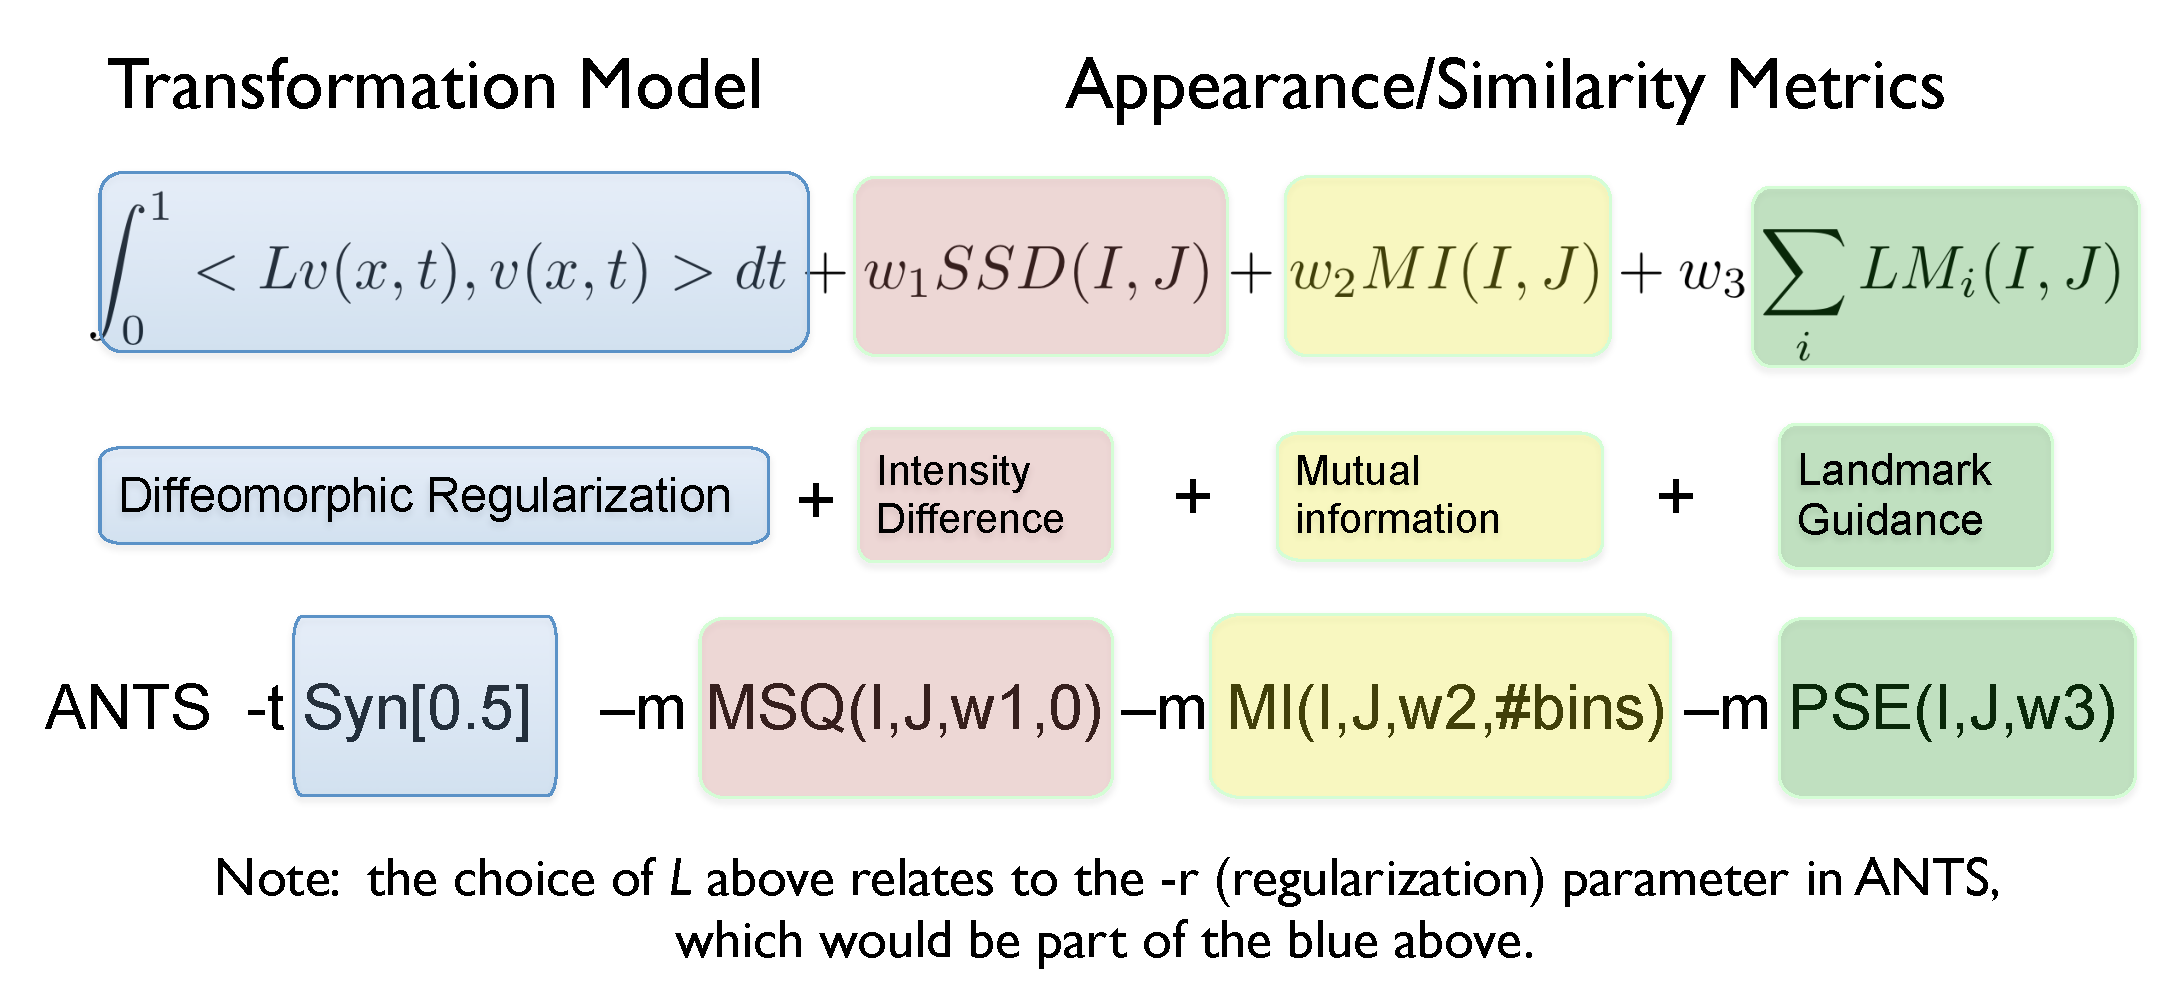
\includegraphics[width=0.9\textwidth]{Figures/ANTSSyntax.pdf} 
\itkcaption[ANTS Command Line]{The relationship between the variational 
form that defines the optimization goals and the ANTS command line.}
\vspace{-0.1in}
\end{figure}
ANTS may be used to navigate the transformation and similarity metric space. 
\subsection{Use Your Header!} ANTS uses the direction/orientation, spacing
and origin in its definitions of the mapping between images.  That is,
ANTS uses the nifti standard defintions of an image space.  So, the
image orientation (direction), origin and spacing are important!  You
may ``check'' for consistency between two image header definitions by
using: ImageMath 3 Image2repaired.nii.gz CompareHeadersAndImages
Image1.nii.gz Image2.nii.gz \newline This will compare Image2 to
Image1 and ``fix'' the header of Image2, writing out to
Image2repaired.


\subsection{ANTS Transformation Models}
The ANTS toolkit provides a hierarchy of transformations with
adjustable levels of complexity, regularization, degrees of freedom
and behavior as optimizers.  The simplest transformation model is the
rigid and/or affine transform.  The most complex -- and most flexible
-- is a symmetric diffeomorphic transformation based on optimizing and
integrating a time-varying velocity field.  Computation time also
increases with transformation model complexity, but most normalization
needs may be met with under an hour of computation.  
We provide an overview of some of the ANTS models below and 
try to communicate intuition on what one gains/loses with each choice.  
An overview of available models and similarity terms is in Table~\ref{table:chart}.
\begin{table*}
  \centering
    \begin{tabular}{c c c c}
    {\bf Category} & {\bf Transformation, $\phi$} & {\bf Similarity Measures} & {\bf Brief Description} \\
    \toprule     
    \multirow{2}*{\bf Linear}
           & Rigid$^\dagger$ & MI, MSQ & Rigid registration. \\
       {} & Affine$^\dagger$ & MI, MSQ & Affine registration. \\
       \cmidrule(l){2-4}
    \multirow{2}*{\bf Elastic}
           & Deformable & CC, PR, MI, MSQ, PSE & Demons-like algorithm. \\
       {} & DMFFD & CC, PR, MI, MSQ, PSE  & FFD variant. \\
       \cmidrule(l){2-4}
    \multirow{2}*{\bf Diffeo.}
           & Exponential$^\dagger$ &  CC,PR, MI, MSQ, PSE  & $~\min~\velocity(\x)$ \\
       {} & Greedy SyN$^\dagger$ &  CC, PR, MI, MSQ, PSE  & ~~locally in time~$\min~\velocity(\x,t)$\\
       {} & Geodesic SyN$^\dagger$ &  CC, PR, MI, MSQ, PSE  &  $~\min~\velocity(\x,t)$ over all time \\
    \bottomrule
    \end{tabular}
  \caption{Transformations and a subset of the similarity metrics available in ANTS.  Similarity metric acronyms:  CC = fast cross correlation, PR = pure cross correlation (the preferred metric), MSQ = mean squared difference, MI = mutual information, PSE = point-set expectation.  ANTS also provides the inverse of those transformations denoted by the `$\dagger$' symbol.  The brief descriptions of the diffeomorphic algorithms contrast the way in which the velocity field is optimized and used to parameterize $\phi$, the mapping.  All 
ANTS Diff algorithms generate $\phi(\x,t)$ over $t \in [ 0, 1]$ through gradient descent.}
  \label{table:chart}
\end{table*}    
\vspace{0in}

\subsubsection{Linear Registration}
\begin{figure}
\label{fig:aff}
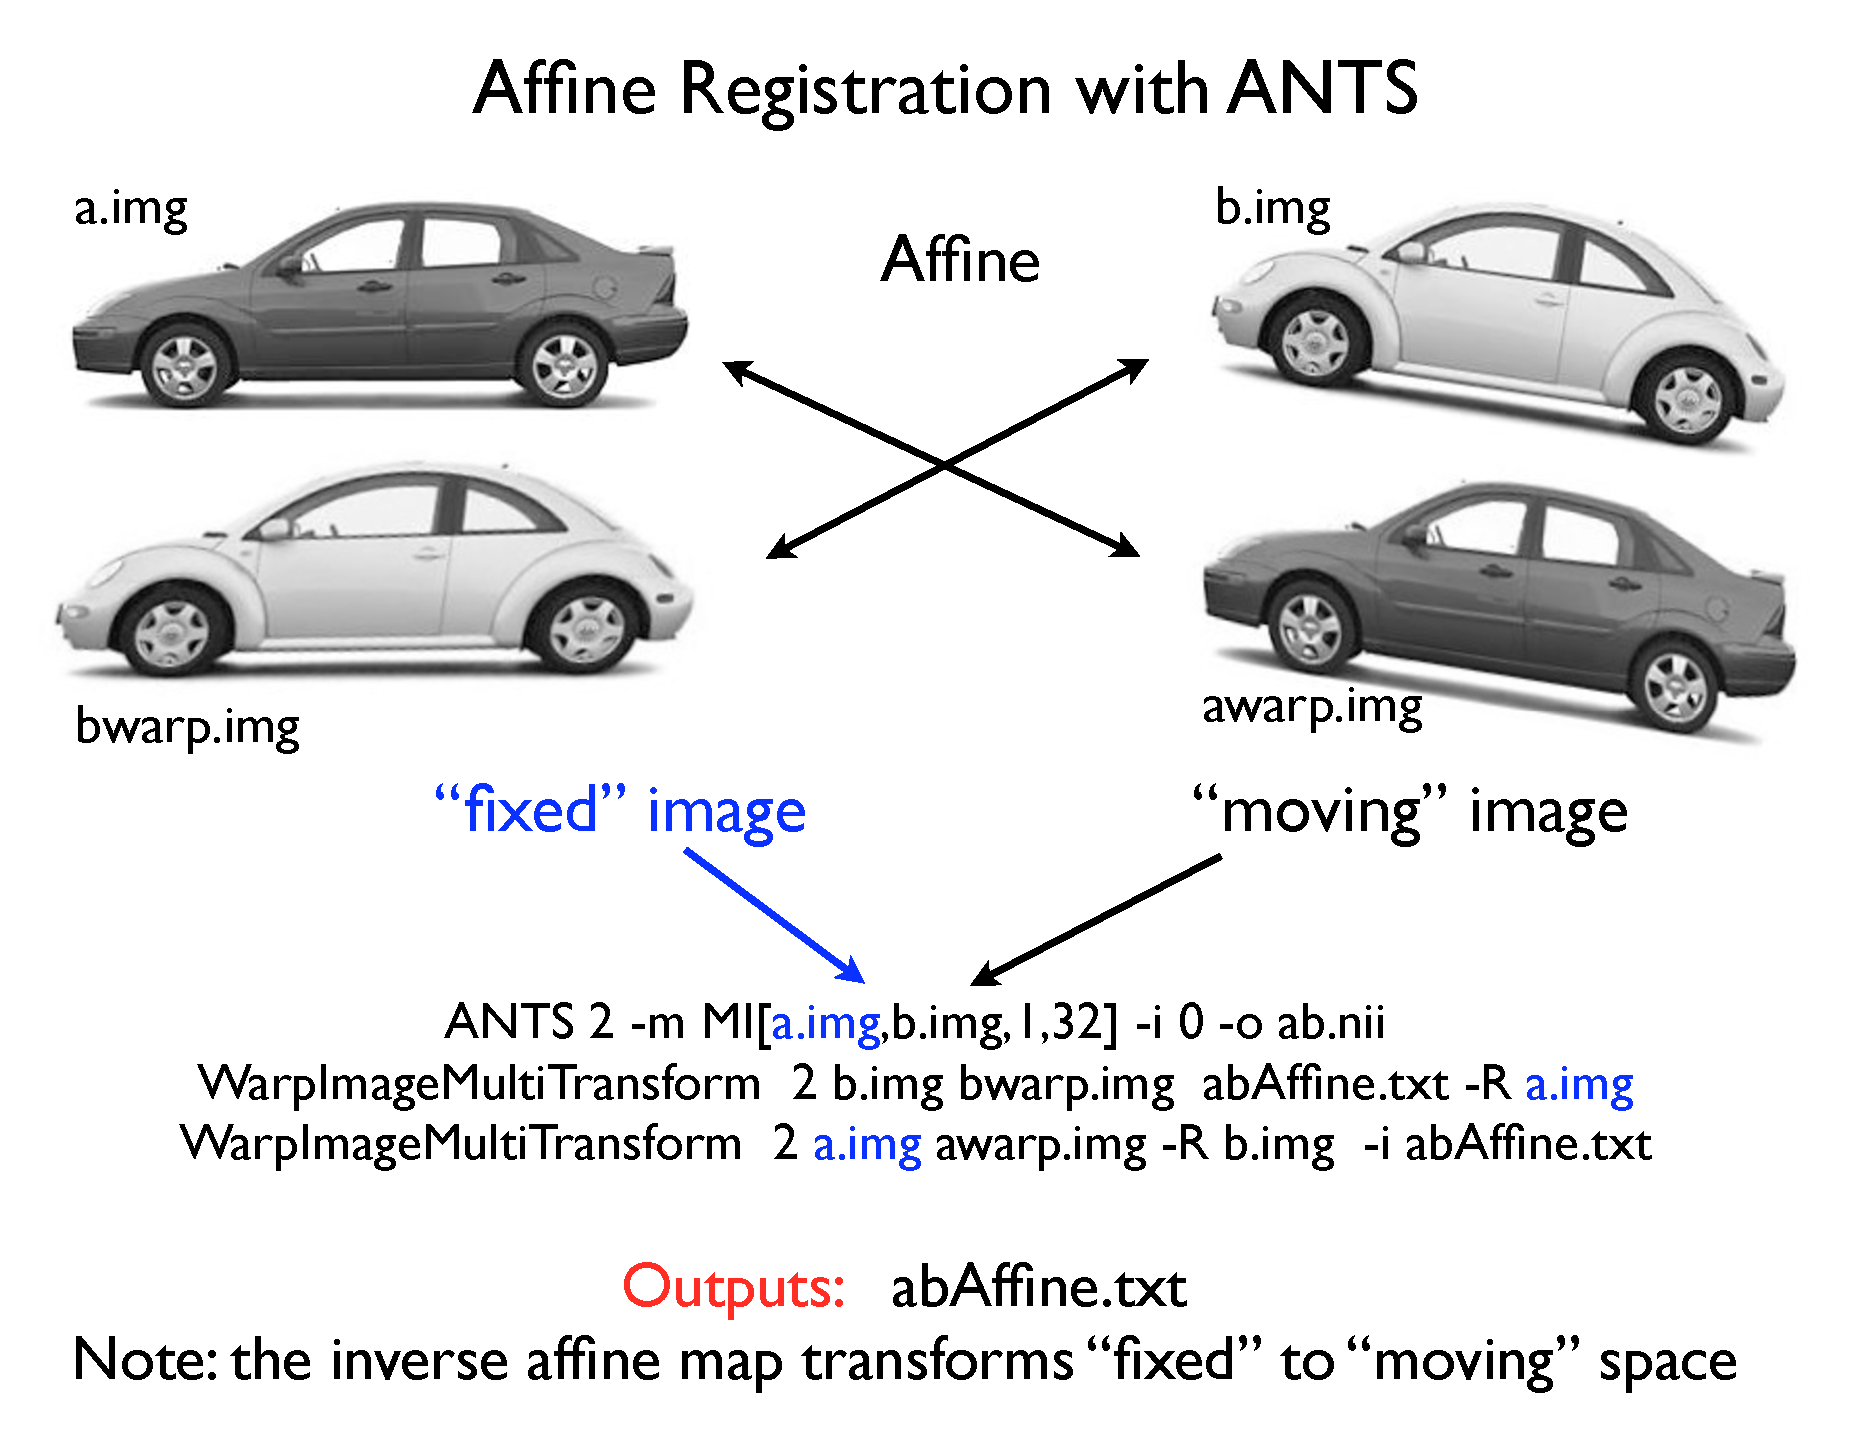
\includegraphics[width=0.9\textwidth]{./Figures/ANTSanatomy.pdf} 
\itkcaption[ANTS Introduction]{The anatomy of an ANTS optimization and application of the resulting warping.}
\vspace{-0.1in}
\end{figure}
The most basic mapping between images is an affine mapping. The ANTS 
affine mapping syntax is shown in the affine mapping figure~\ref{fig:aff}. The
parameter breakdown of the ANTS call in the affine figure is:
\begin{itemize}
\item  ANTS -- the normalization program
\item 2 -- the expected image dimension
\item -m MI[...,...,1,32] -- the similarity metric "mutual information" with a 32-bin square joint histogram and weight of 1.  
Metric details will be discussed in a later section. 
\item -i 0 -- no deformable iterations (affine only).
\item -o ab -- the output prefix.  A specific extension may also be specified, e.g.   -o ab.mhd  .
\end{itemize}
The parameter breakdown of the WarpImageMultiTransform call in the affine figure is:
\begin{itemize}
\item WarpImageMultiTransform -- to apply the mapping output from ANTS to an image.
\item 2 -- the expected image dimension.
\item the image to be deformed is input next.
\item the deformed image output file name is next.
\item the transform itself is next -- if is affine and preceded by " -i ", we apply the inverse affine map.
\item the " -R " option dictates the domain you want to warp into -- usually the ``fixed'' image, unless using the inverse mapping, in which case one switches the role of fixed and moving images. 
\end{itemize}
Note that -i 0 (in the ANTS call) means that no deformable mapping is performed. The call "ANTS 2" means to treat the images as 2-dimensional. "ANTS 3" would be called for 3D images. The " -m " term defines the similarity metric. 
Note that no more than one image interpolation is used during optimization.  
That is, ANTS always references the original image before applying a transformation or series of transformations. 

Affine mapping may become nontrivial when the region of interest 
occupies only a small portion of the image data.  In such cases, 
ANTS enables the user to define a mask to focus the optimization 
effort on the region of interest.  
Example code for (affine) registration with a mask: 
\begin{verbatim}
ANTS 3 -m MI[AtlasHead.nii,crAnatomical.nii,1,32] 
-o TEST -i 10x10x0  -r Gauss[1.5,0] -t Exp[0.5] -x mask.nii.gz
\end{verbatim}
The difference between this command 
and a regular ANTS call is the \verb"-x" option, which specifies the mask, defined in the 
template space (here, AtlasHead.nii).   The mask option also affects the deformable optimization. 
Other affine registration options include  \verb"--number-of-affine-iterations 5000x5000x5000" which specifies that the affine registration uses a 3 level image pyramid with each level 5000 iterations at most. \verb"--MI-option 48x6000" means to use Mutual Information as similarity metric with 48 bins and 6000 samples. \verb"--affine-gradient-descent-option" defines the options for the gradient descent procedure; the 4 numbers are maximum step length, relaxation factor, minimum step length and translation scale.  

\subsubsection{Deformable Registration}
Affine mapping is adequate when the
difference between images involves only rotation, scaling or shearing.
Other data requires more deformable mappings to capture shape
differences and find a good alignment of image features.
Figure~\ref{fig:antshier} shows how deformable mapping may improve the
correspondence of the deformed beetle to the ford image.
\begin{figure}
\label{fig:antshier}
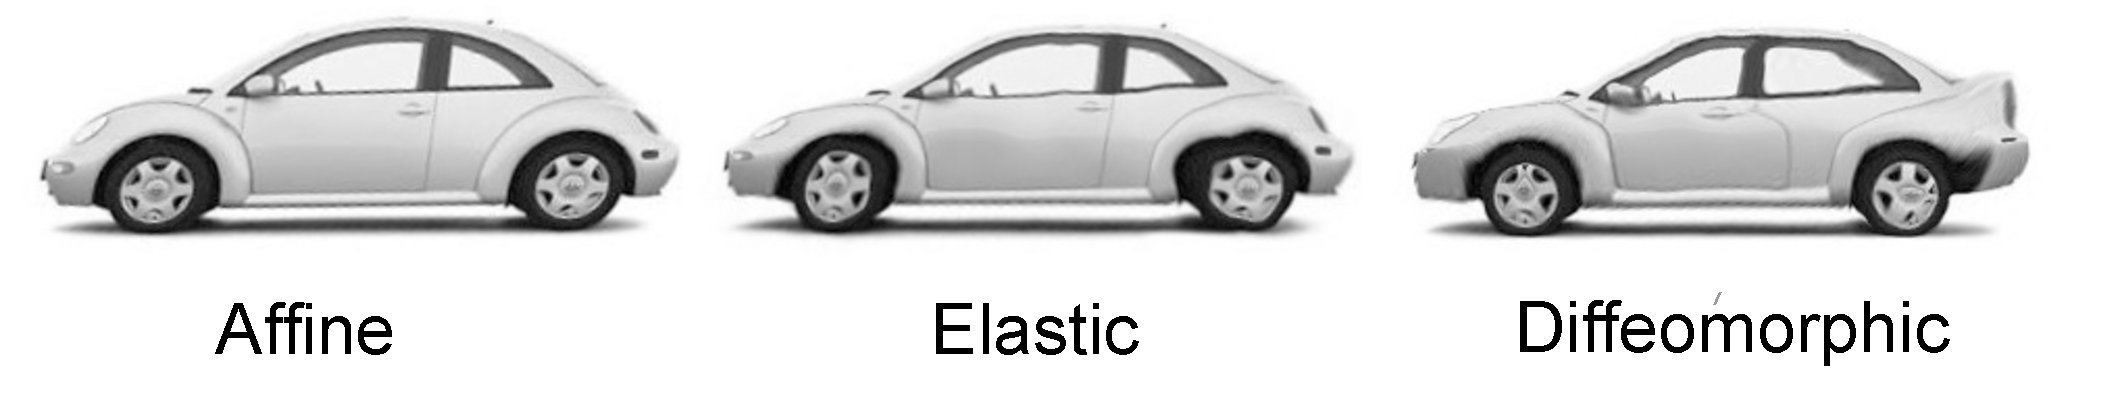
\includegraphics[width=0.9\textwidth]{./Figures/ANTSElastToDiff.pdf} 
\itkcaption[ANTS Transformation Examples]{This example shows the degree to which the beetle (b.img) may be deformed to the ford (a.img) under different transformation models.  Left to right increases the degrees of freedom in the mapping and thus the registration accuracy.}
\vspace{-0.1in}
\end{figure}
Most ANTS-based applications use symmetric diffeomorphic normalization.  However, 
ANTS also enables a simpler parameterization of a deformable mapping via a regularized 
vector space.  We term these types of transformations as ``elastic''.  The original Demons algorithm 
provides a classic example of using a regularized vector space for nonlinear registration.  
Caveats are that a regularized vector space may not preserve the underlying topology 
and may also prove too inflexible to capture the shape changes one is after.  Both of these 
shortcomings motivate the use of diffeomorphisms. 

\noindent{\bf Elastic/Vector Space Transformations.} If we assume no affine transformation, then 
an elastic transformation involves computing a mapping from image $I(\x)$ to image $J(\x)$ 
through a deformation field $\disp( \x )$.  
\begin{wrapfigure}{r}{0.5\textwidth}
\label{fig:pull}
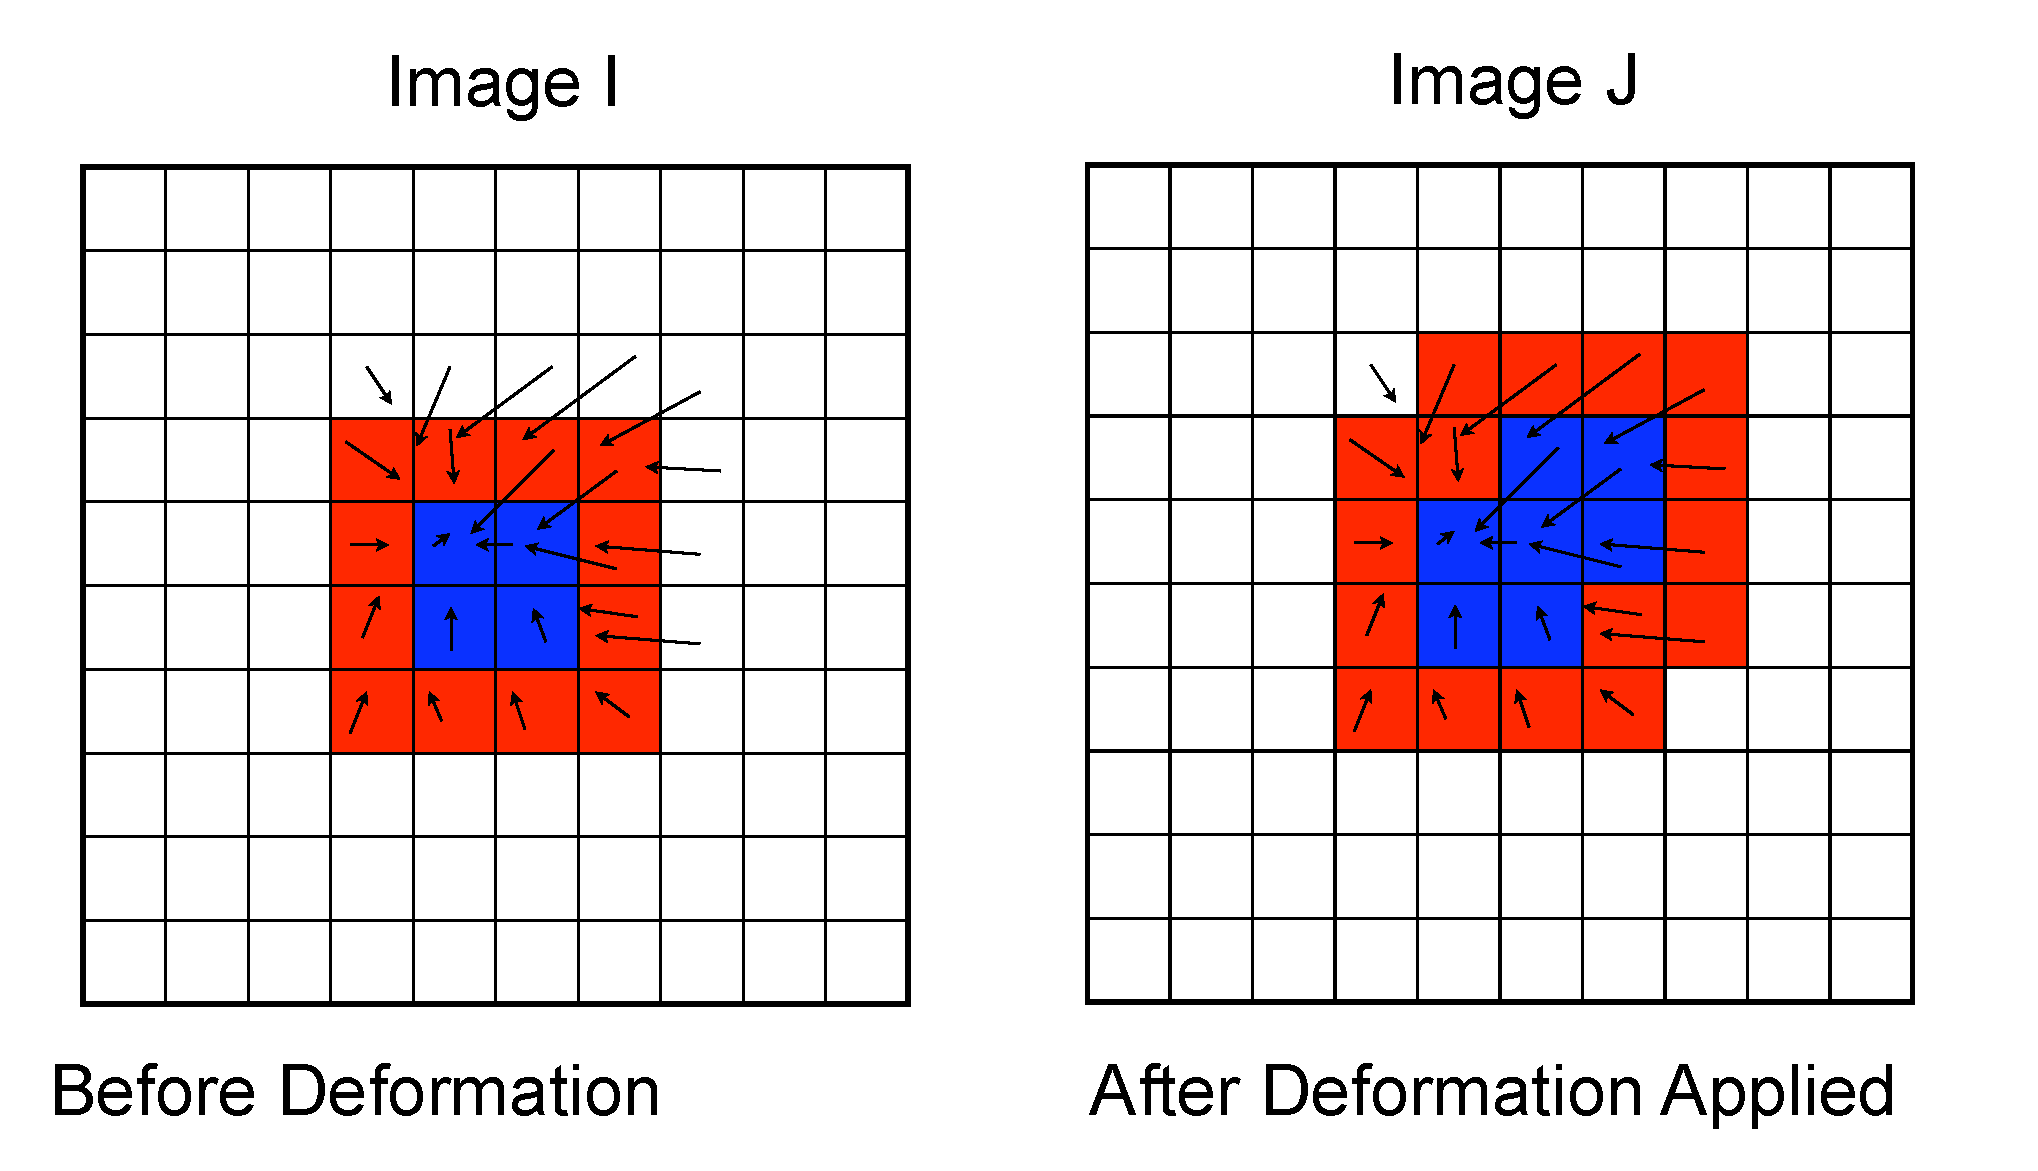
\includegraphics[width=0.45\textwidth]{./Figures/PullBack.pdf} 
\end{wrapfigure}  
The deformation is defined in the physical space of the image 
and dictates the positional difference between corresponding features in the two images.  
Thus, if a feature defined at $I(\x)$ matches a feature in $J$ at position $\y$ then the deformation 
field at $\x$ should give $\disp ( \x )=\y-\x$.   
Such a deformation field may be applied to deform 
image $J$ into image $I$ by composing the mapping $J_{deformed}(\x)=J(\x+\disp(\x))$.  
In a perfect world, then $I(\x)=J_{deformed}(\x)$, though this is rarely the case.  Figure~\ref{fig:pull} 
visualizes the deformation of an image under this standard model. 
Gradient descent optimization of an elastic mapping may be summarized (crudely) as: 
\begin{align}
\text{Compute the similarity gradient:   }  \nabla E = \partial_{\disp} \Pi(I,J(\x+\disp(\x))). \nonumber \\
\text{Update the deformation field:  }  \disp(\x) \leftarrow \disp(\x)+\delta \nabla E. \nonumber \\ 
\text{Regularize the deformation field:  }  \disp(\x) \leftarrow G_\sigma \star \disp(\x),
\end{align}
where $\Pi$ is the similarity, $\delta$ is a gradient step length and $G_\sigma$ is a gaussian smoother.
This optimization is captured in the following ANTS command:
\begin{verbatim}
ANTS 3 -m PR[AtlasHead.nii,crAnatomical.nii,1,4] -r Gauss[0,3]  
-o ElasticTest.nii.gz -i 30x20x10  -t Elast[1.5] 
\end{verbatim}
Here, we use the PR metric (a cross-correlation implementation) with
window radius 4, weight 1 and gradient step length 1.5.  The
optimization will be performed over three resolutions with a maximum
of 30 iterations at the coarsest level, 20 at the next coarsest and 10
at the full resolution.  We use a Gaussian regularizer with a sigma of
3 that operates only on the deformation field and not on the similarity gradient, as 
0 is passed as the first parameter to \verb Gauss .  One may see the
correspondence, yet again, between the ANTS call and the optimization
scheme.  The optimization will stop when either the energy cannot be 
smoothly minimized or the maximum number of iterations is reached. 
BSpline regularization is also available in ANTS -- see the DMFFD 
section below.  

\noindent{\bf Warping and Invertibility.}  ANTS uses physical space to
define mappings. The origin etc is in the coordinates of the world in
which the picture (e.g. MRI) was taken. Then, warping between physical
coordinates is relatively easy. Differences in bounding boxes etc
present no problem -- assuming you avoid inconsistent headers
i.e. origins, directions, data orientation. One may use PrintHeader to
check the data and run simple, fast tests (few iterations) to perform
sanity checks before running through loads of data.
An ANTS deformation consists of
a standard naming prefix plus a standard naming extension. We usually 
assume nii but other file types may be used. The standard naming
extension is Warpxvec.nii for the x component of the deformation with
similar naming for y and z. Each component is stored in a separate
scalar image. The value of a voxel of a deformation/warp component
image is the physical space displacement from that voxel. Note that
the inverse mapping is stored in InverseWarpxvec.nii and provides the
mapping in the opposite direction.  Note that an inverse -- in the 
digital domain -- is only approximate as shown in figure~\ref{fig:inv}.
\begin{figure}
\label{fig:inv}
\center 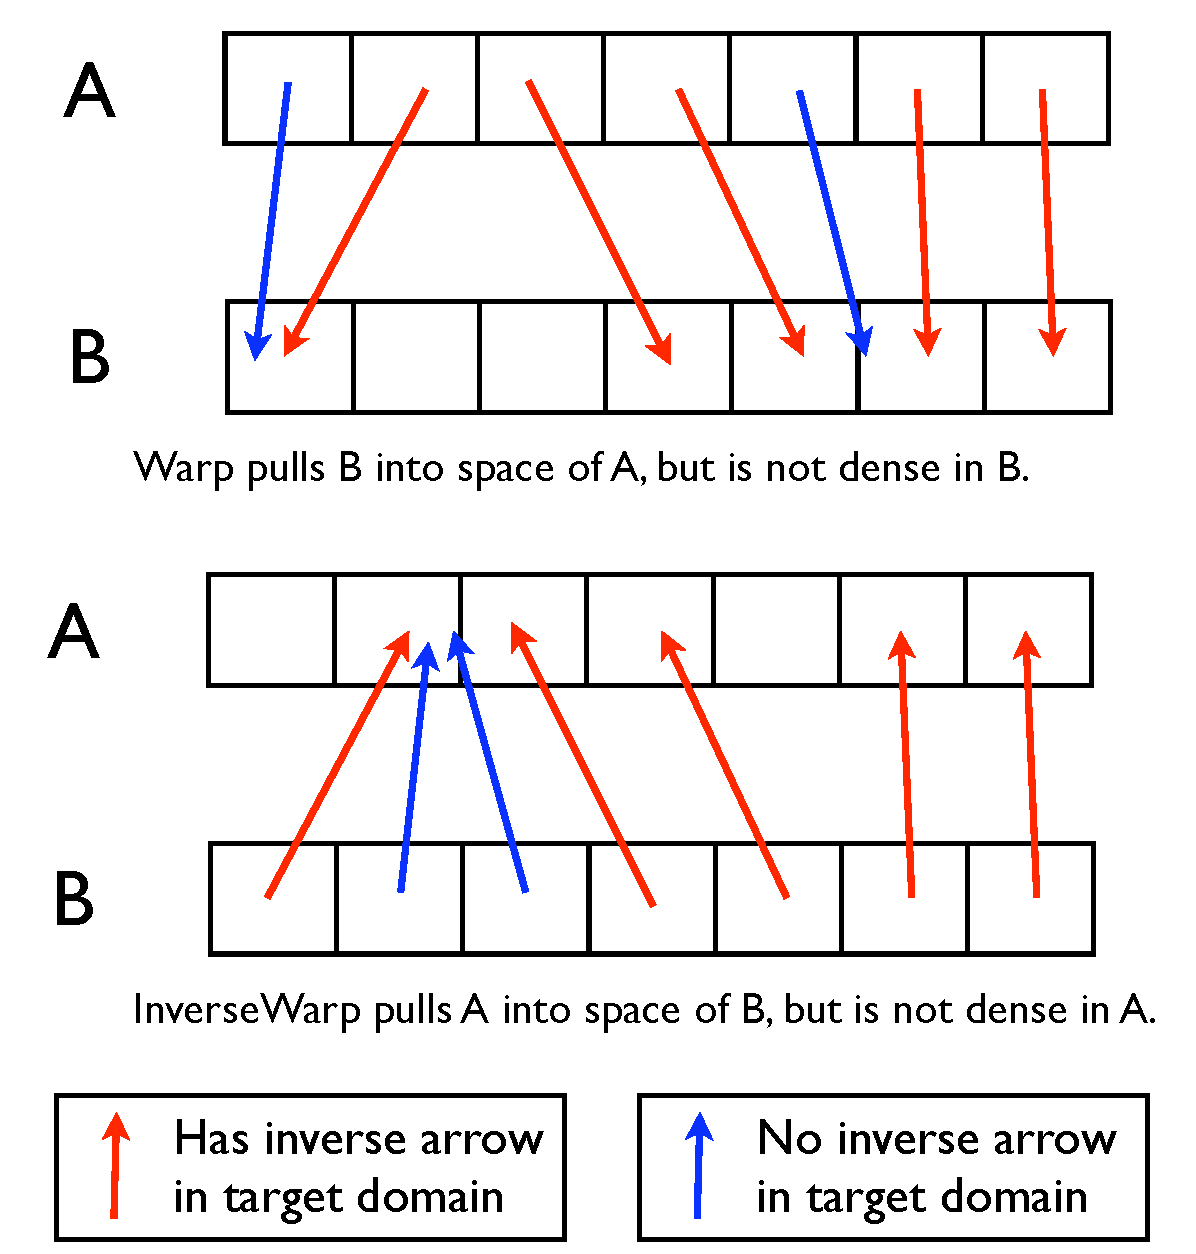
\includegraphics[width=0.75\textwidth]{Figures/DeformationsInDigitalDomain.pdf} 
\itkcaption[Digital Invertibility]{Digital invertibility presents some limitations. 
Here, we see that invertibility is not exact but is gained only by interpolation.  
Thus, in three-dimensional scenarios in particular, there are fundamental limits to the 
degree of invertibility that may be achieved.  The second and third voxels -- from left -- 
in image A undergo an expansion by a factor of 2.  That is, under the mapping, 
2 voxels are mapped to 4.  This gives the definition of the Jacobian -- computed 
by  ANTSJacobian -- which is a unitless measure defined by the 
ratio of volumes.  Thus, $\mathcal{J}(\x)=V(\phi(\x))/V(\x)$ where $V$ represents 
the volume operation and $\x$, here, may be a small object.  Thus, if $\phi$ -- the mapping -- 
causes expansion, then $\mathcal{J}(\x) > 1$. }
\vspace{-0.1in}
\end{figure}  
A few important notes follow. 
(1) Deformation directionality: Warps/deformations applied to images occur in the opposite direction from warps/deformations applied to points. That is, if we map image B to A using 
\begin{verbatim}
ANTS 2 -m PR[A,B,1,2] -o OUTPUT 
\end{verbatim}
 then we get a deformation called \verb OUTPUTWarp+extensions ~and an affine transform called \verb OUTPUTAffine.txt . 
This composite mapping - when applied to B - will transform B into the space of A. 
However, if we have points defined in B that we want to map to A, 
we have to use \verb OUTPUTInverseWarp ~and the inverse of \verb OUTPUTAffine.txt .  
This is because the domain and range of the map's definition need to be dense in a way that is appropriate for the data type. 
Figure~\ref{fig:inv} illustrates the concept. 
(2) Older Image Formats: older image formats (e.g. Analyze) may not
have proper origin/offset/direction support! In these cases, we
recommend converting to nii and verifying that data overlays properly.
(3) Transorm Composition: Composition of transforms may be achieved with
ComposeMultiTransform.  (4) Warping with inverses and concatenations --
viable when using diffeomorphisms -- are described in
figure~\ref{fig:warp}.
 \begin{figure}
\label{fig:warp}
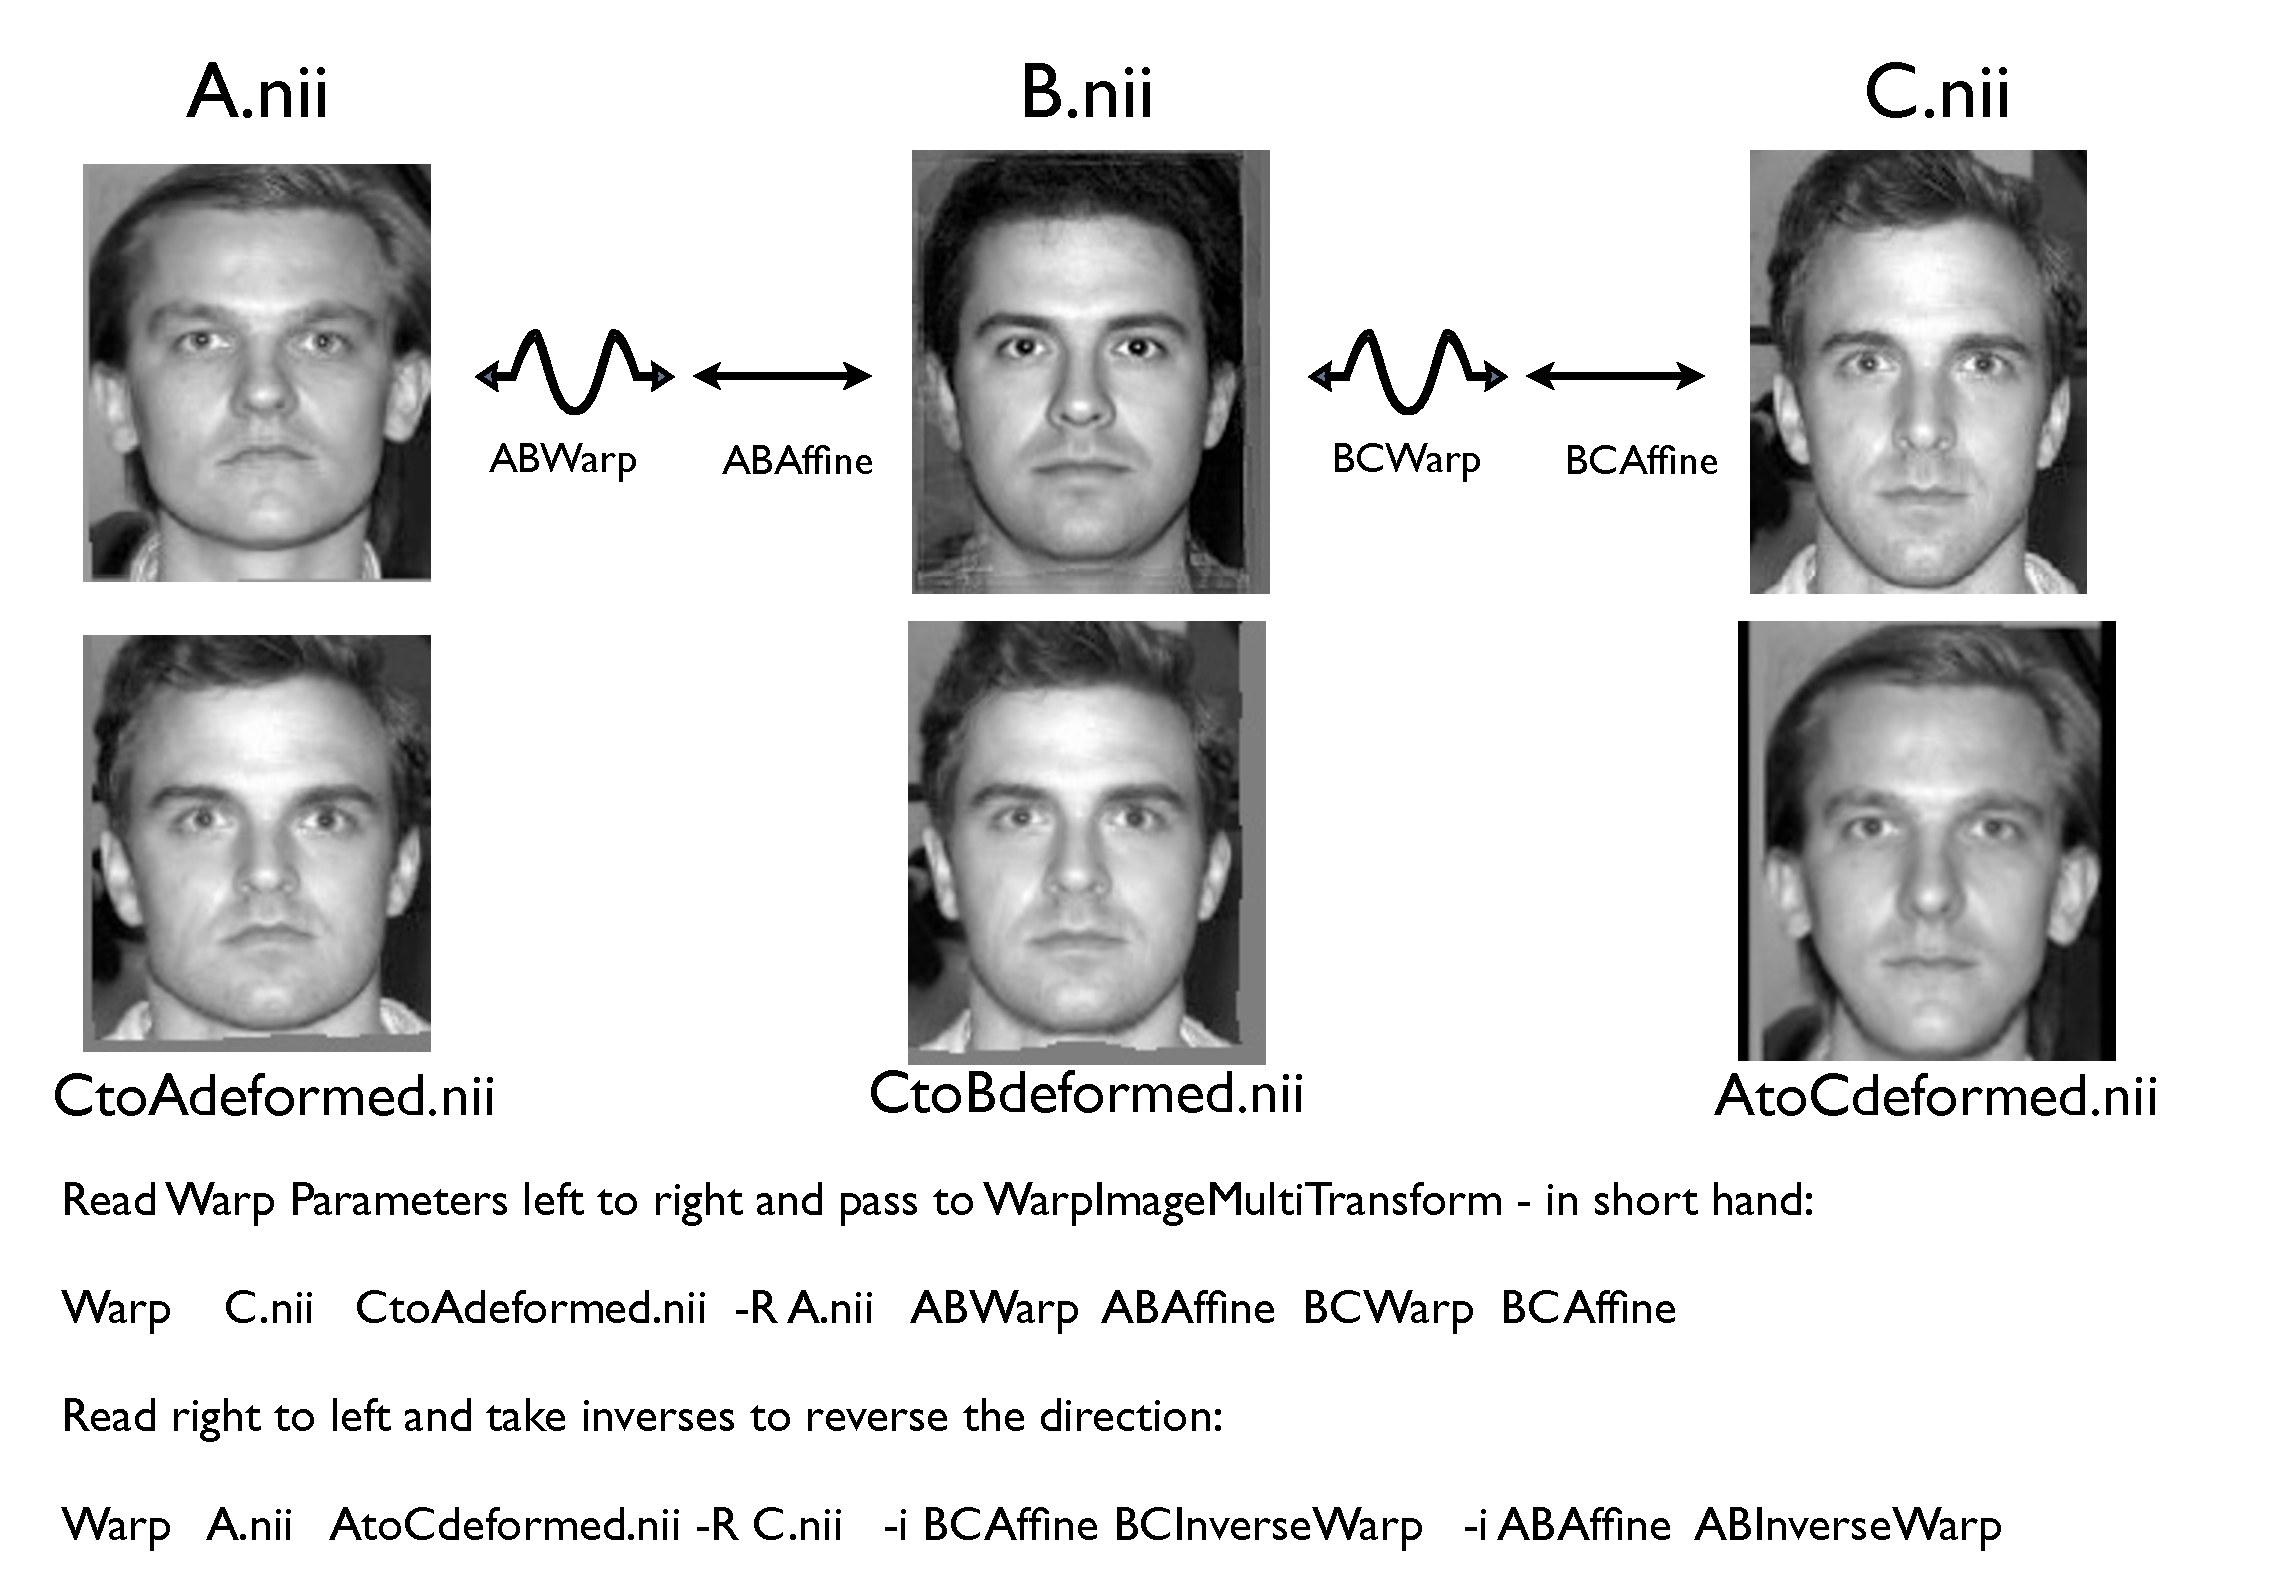
\includegraphics[width=0.9\textwidth]{Figures/ANTSSyntax2.pdf} 
\itkcaption[ANTS Warping]{Here, we detail how one applies 
a deformation and associated inverses.  We also see how 
WarpImageMultiTransform can be used to concatenate a series 
of transformations.}
\vspace{-0.1in}
\end{figure}

\noindent{\bf Diffeomorphic Transformations.}  The elastic 
mapping space -- as indicated above -- may prove inadequate 
for some large deformation mapping scenarios.  Figures~\ref{fig:antshier} 
illustrate the changing performance one may get in switching from affine 
to elastic to diffeomorphic normalization.  
\begin{figure}
\label{fig:antssyn}
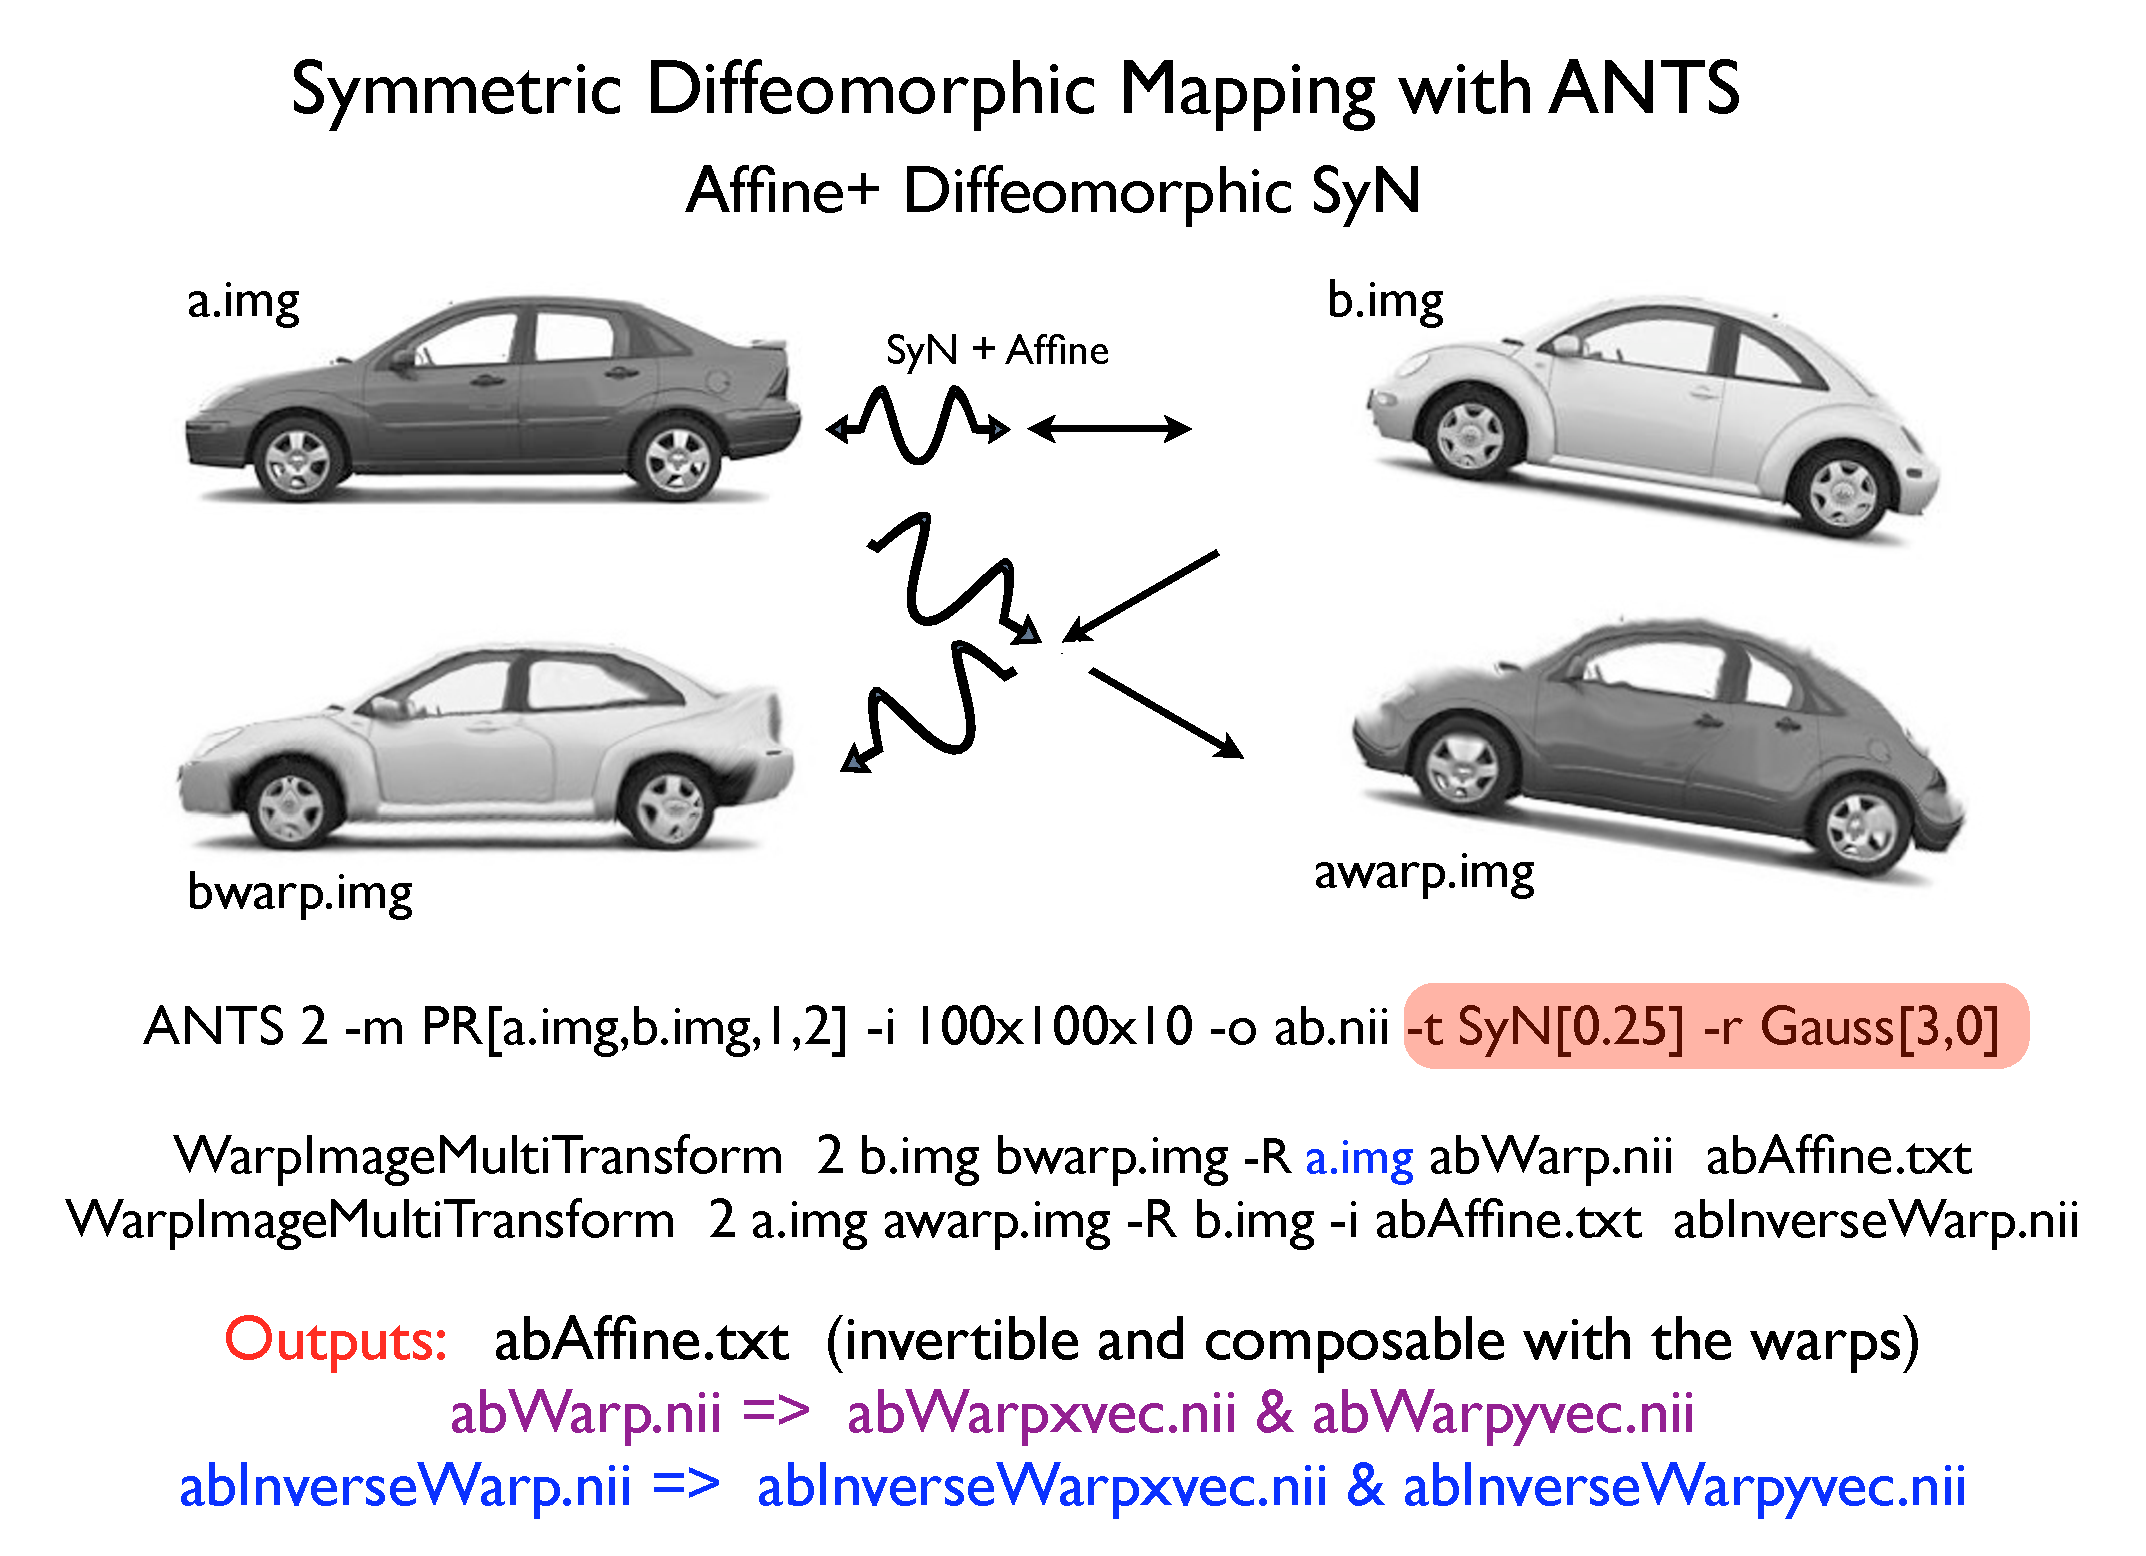
\includegraphics[width=0.9\textwidth]{./Figures/ANTSsyn.pdf} 
\itkcaption[ANTS Symmetric Normalization]{This example shows the benefit of the symmetric normalization model -- invertibility, symmetry, highly deformable and accurate registration.  The transformation model used here is highlighted in red.}
\vspace{-0.1in}
\end{figure}
Figure~\ref{fig:antssyn} shows 
how one may use ANTS to achieve a state-of-the-art diffeomorphic mapping. 
The ANTS diffeomorphic model chosen for this example -- symmetric normalization -- 
is invariant to the order of the input images (although the affine mapping is not).  
An additional advantage of the diffeomorphic model over the elastic model is 
that both forward and inverse transformations are computed thus allowing one 
to deform fixed to moving and also moving to fixed.   The transformation model 
chosen here -- \verb SyN[0.25] -- may be replaced with other 
diffeomorphic transformation models.  The most general is global-in-time SyN via \verb SyN[0.25,2,0.01]   , 
where the time step for integration is 0.01 (lower is more accurate).  A fast approximate 
solution may be gained through 
exponential mapping via \verb Exp[0.25,10] , where 10 integrations points are used. 
Update schemes for diffeomorphic optimization are similar to the elastic case 
and are described elsewhere \cite{Avants2008b,ANTStheory}.   

\subsection{ANTS Similarity Terms}
Here is a script that will let you experiment with different similarity term 
and transformation model combinations.  A few are listed, with parameters 
that are a reasonable starting point.
\begin{verbatim}
II=r16slice.nii # change to your own images 
JJ=r64slice.nii 
DIM=2 # two-dimensional images 
ITS=" -i 100x100x30 " # 3 optimization levels 
TSYNWITHTIME=" -t SyN[1,2,0.05]  -r Gauss[3,0.5] "
TGREEDYSYN=" -t SyN[0.25]  -r Gauss[3,0] "
TELAST=" -t Elast[1] -r Gauss[0,3] " 
TEXP="  -t Exp[0.5,10] -r Gauss[0,3] " 
LABELGUIDED=" -m PSE[${II},${JJ},${II},${JJ},0.75,0.1,25,0,10] "
INTMSQ=" -m MSQ[${II},${JJ},1,0.1] "
INTMI=" -m MI[${II},${JJ},1,32] "
INTPR=" -m PR[${II},${JJ},1,4] "
NAME=TEST
INT=$INTPR
TRAN=$TSYN
ANTS $DIM -o $NAME $ITS  $TRAN  $INT
INVW=" -i ${NAME}Affine.txt ${NAME}InverseWarp.nii "
FWDW=" ${NAME}Warp.nii ${NAME}Affine.txt "
WarpImageMultiTransform  2 ${II} a.nii -R ${JJ} $INVW
WarpImageMultiTransform  2 ${JJ} b.nii -R ${II} $FWDW
\end{verbatim}
Convergence occurs under two conditions: (1) either the maximum number of 
iterations are reached at a given optimization level or (2) the slope 
of the change in the optimization objective is negative or very small. 
{\em Note: ANTS does not like spaces between brackets in the call to the metrics.}

\subsection{Diffusion Tensor Normalization}
The ImageMath program -- via TensorFA and TensorMeanDiffusion -- 
may derive scalar images from DTI.  Such images may be used to 
distortion correct DTI to T1 or to map DTI together.   See the 
ANTS/Scripts program called \verb antswithdt.sh ~for a 
ready to go example.   Figure~\ref{fig:dterr} shows what might 
happen if your tensor entries are stored in the wrong order. 
ANTS expects the nifti standard ordering of the DT six vector.
\begin{wrapfigure}{r}{0.5\textwidth}
\label{fig:dterr}
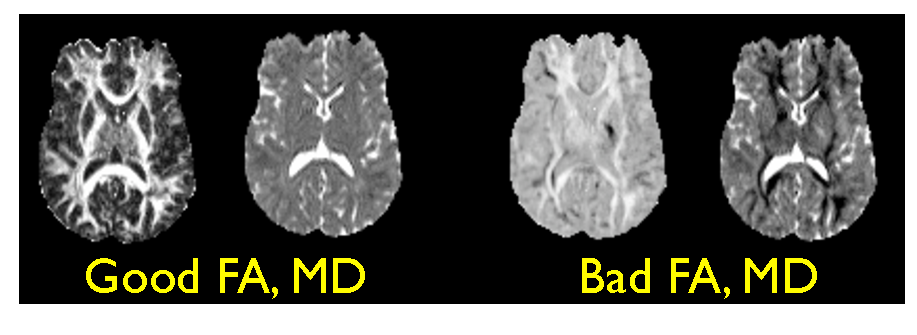
\includegraphics[width=0.5\textwidth]{Figures/dtiordererr.pdf} 
\itkcaption[DT Entry Error]{The FA and mean diffusion of the tensor may be corrupted, 
as at right, if the order of the DT entries is wrong.}
\vspace{-0.1in}
\end{wrapfigure}  
\subsection{Multivariate Normalization with ANTS}
\begin{figure}
\label{fig:mvnorm}
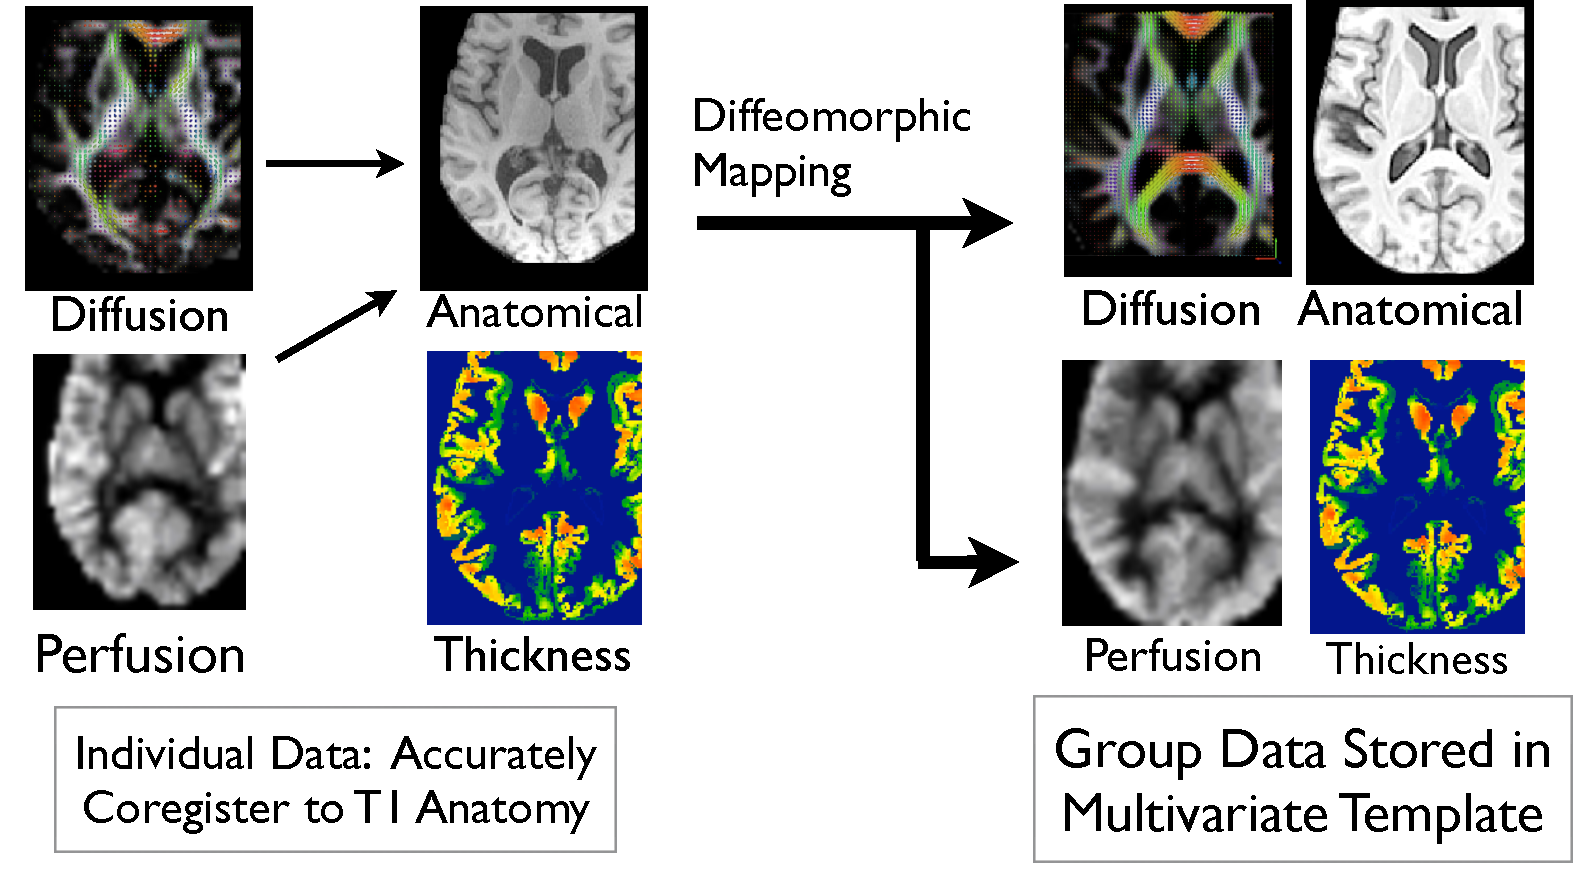
\includegraphics[width=0.9\textwidth]{Figures/multivariatenorm.pdf} 
\itkcaption[Multivariate Normalization]{The current version of ANTS 
may perform normalization of multiple modalities by combining {\em intrasubject, intermodality} mappings with {\em intersubject, intramodality} maps to a 
group template.  In brain imaging, the intersubject maps are usually guided by the T1 component.}\vspace{-0.1in}
\end{figure}
Multivariate normalization may be performed in two ways with ANTS.  
First, as shown in figure~\ref{fig:mvnorm}, intra-subject mappings may 
be used to conform all modalities into a common subject space defined by 
the ``anchor'' modality.  In brain imaging, this is usually the T1 component.  

A second type of multivariate normalization is able to use the T1 and DTI components 
directly in the optimization of the mapping.  An example of this type of call is below, 
where we assume that one has resampled the DT data to the space of T1: 
\begin{verbatim}
ANTS 3 -m PR[T1template.nii,T1subject.nii,1.25,4]
       -m PR[FAtemplate.nii,FAsubject.nii,1,4] 
-o MultiVar -i 30x30x20  -r Gauss[3,0] -t SyN[0.25]
\end{verbatim}
In this case, dense features within white matter are gained by using the DT component  
in addition to the T1 component.   The T1 PR metric, here, is weighted slightly more 
than the FA PR metric, 1.25 vs. 1.0.  {\em The convergence criterion for 
the multivariate scenario is a slave to the {\bf last} metric you 
pass on the ANTS command line}.

\subsection{Optimal Template Construction with ANTS}
A useful script for setting up optimal template construction
 is available in ANTS/Scripts.  Two versions of available : serial and parallel.  
Data and a script for building an average face template is available 
the ANTS/Examples/Data directory.  Two key points about optimal templates:
1. The outcome stabilizes at around ten images, for most populations.
That is, if we randomly select images from individuals within the same 
demographic distribution, we will end up with very similar average images.  
2.  Optimality, for the ANTS-SyN approach, is defined by the minimum shape 
and appearance distance image. 
See the template page for some examples of this and users may 
contact ANTS developers for previously derived template 
images that may be useful. 

\subsubsection{A Concrete Template Construction Example, Step-by-Step}
For this example, we will use the data in "ANTS/Examples/Data/B*.tiff."
The files are B1.tiff, B2.tiff, B3.tiff, B4.tiff and B5.tiff.   They are single slices 
from a dataset of real MRI brain images -- individuals around 15 years of age. 
Our goal is to derive a "most representative" single image from this population. 
The steps are: \begin{figure}
\label{fig:template}
\center 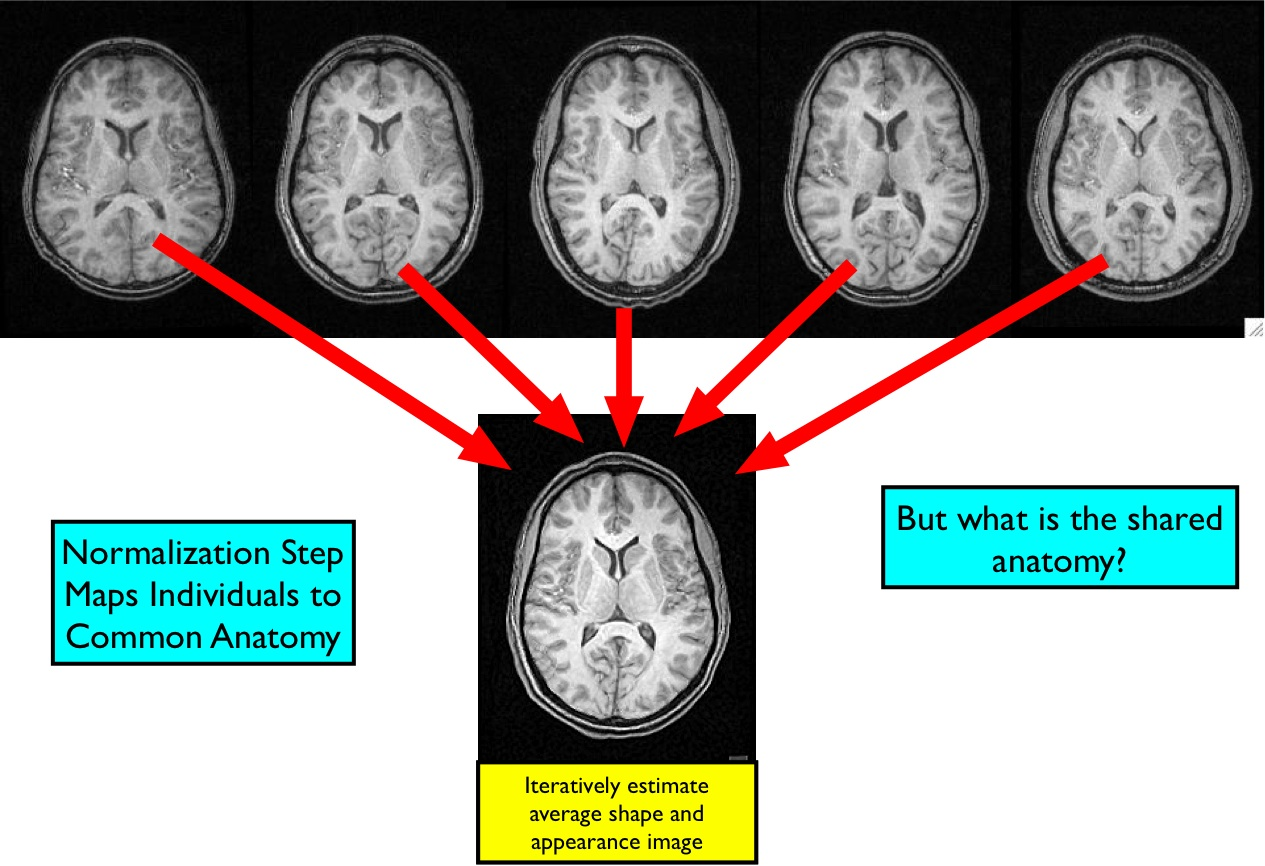
\includegraphics[width=0.7\textwidth]{Figures/templateex.jpg} 
\itkcaption[ANTS Optimal Template]{This example may be recreated by the user.  The shared anatomy -- 
across this dataset -- is recovered in the derived optimal template.}
\end{figure}
\begin{enumerate}
\item   Make a directory for this example.   Copy or link all the B*tiff images into it.
\item Copy the file ANTS/Scripts/buildtemplate.sh into that directory.  
\item  On the command line, within that directory, run the following command: 
\verb  sh ~ \verb buildtemplate.sh ~ to get usage. 
\item If you follow the usage, you will then call the script something like this: 
\verb sh ~ \verb buildtemplate.sh ~ \verb 2 ~ \verb B ~ \verb tiff ~ \verb OUT ~ \verb 4 ~ . 
\item The script should exit and ask if the parameters are ok for your problem.  
Check the path to the programs, the fact that all the images you want to use are being 
listed and that the template output name is ok with you.  
Once everything is prepared, then edit the script to remove the exit call at the end of the parameter check. 
\item  Call the script as in step 4 and then wait for the output.  The template will 
be called something like (in this example)  \verb OUTtemplate.nii .
\end{enumerate}
The script is fairly easy to alter so that you can send the whole thing to distributed computing. 
Typically, one would use voxbo or the qsub program available in the Sun Grid Engine.  This 
is what is done in \verb buildtemplateparallel.sh .  
Figure~\ref{fig:template} shows the data and a result that may be recreated by the user.
\subsection{Notes on Large Deformation Mapping} 
Figure~\ref{fig:large} defines what one might expect from a 
high-resolution, large deformation, successful normalization.  
Major and many minor features are well aligned between 
these images to an extent that is approaching the limits 
allowable by biological variation.  
\begin{figure}
\label{fig:large}
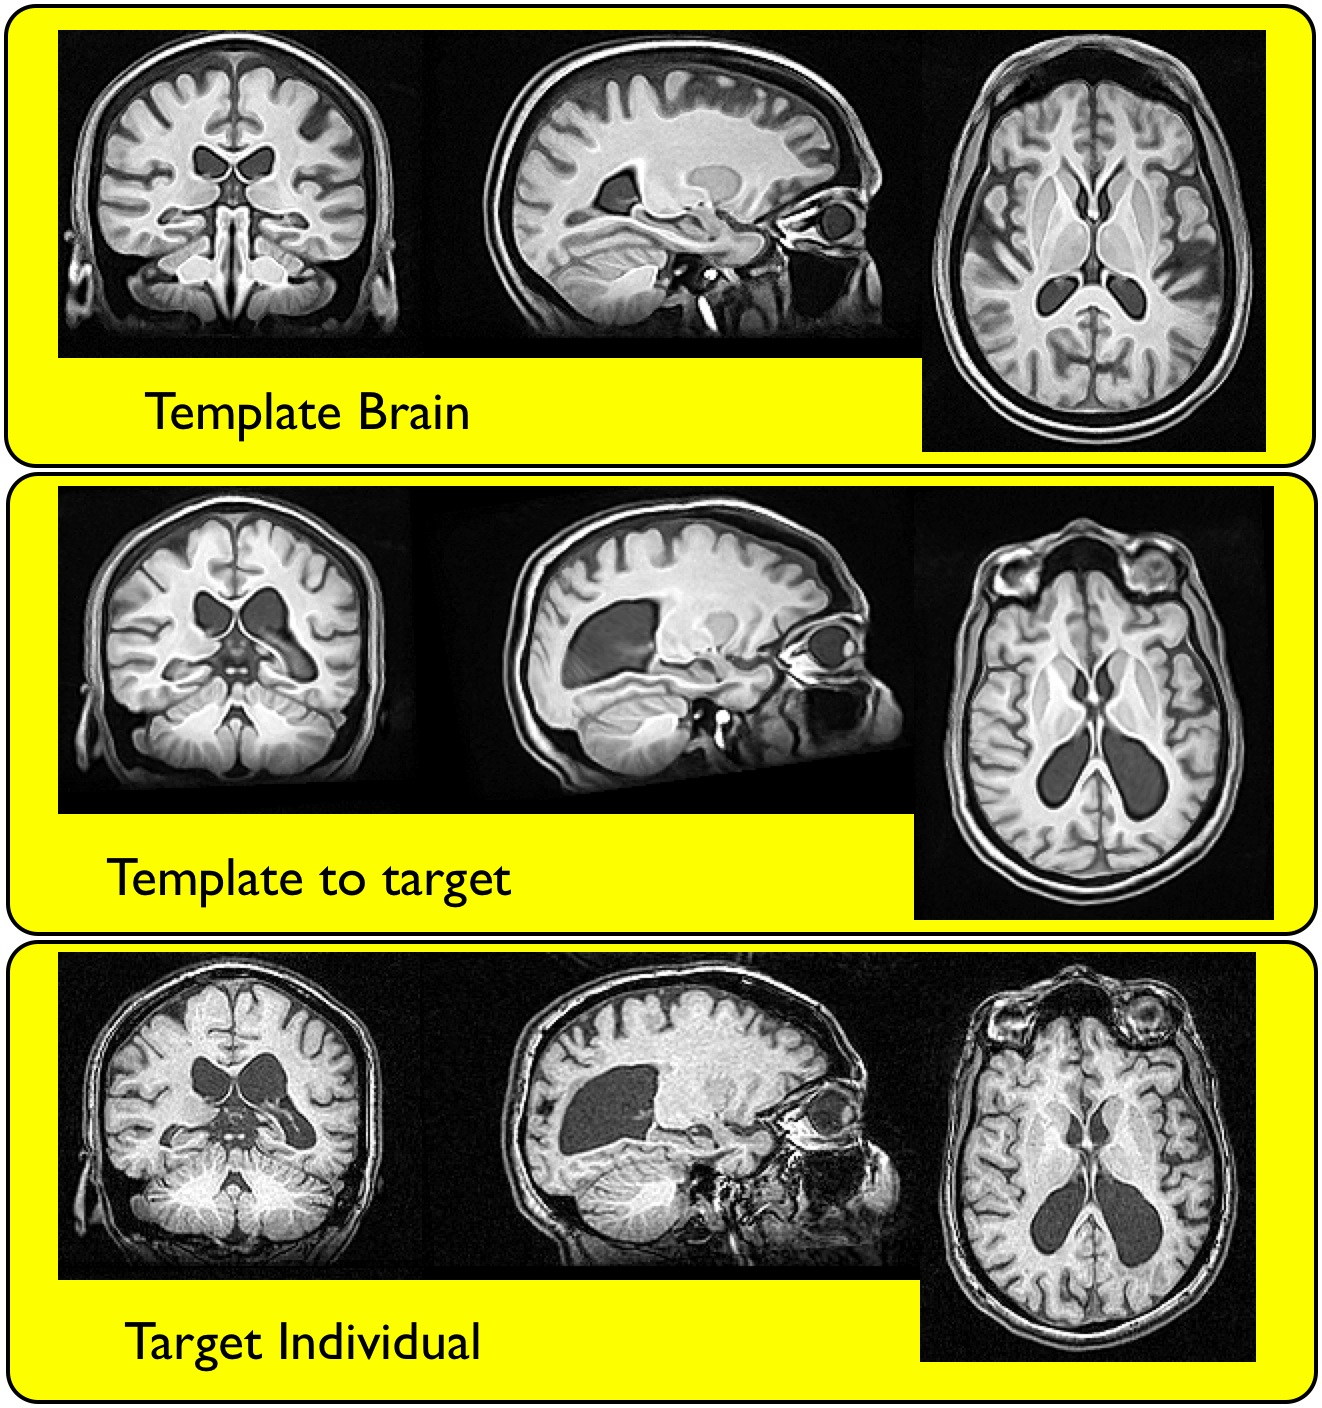
\includegraphics[width=0.9\textwidth]{Figures/ANTSLargeDef.jpg} 
\itkcaption[ANTS LargeDeformation]{ANTS succeeds in a challenging 
normalization scenario.  Comparing the template mapping to the
individual shows that much of the cortex is well-aligned, as is the
hippocampus, despite the relatively large difference between the
initial template and the target.  Here, one might note a limitation of
whole brain mapping: occipital lobe sulcal variation is highly
idiosyncratic and extremely difficult to capture, in particular when
there is such severe atrophy nearby.
}
\end{figure}
\noindent{\bf Turning "Failures" into Successes:} 
Below are some pointers to follow if you are unable to recreate such normalization quality.  
Usually, reasons for registration failure are one of a very few things: 
\begin{enumerate}
\item The initialization is so off mark that affine registration fails -- thus meaning all subsequent deformable registration will not be meaningful.
\item The information within headers is inconsistent e.g. origins are defined in different ways, the "directions" are not correct or some combination of these.    The PrintHeader executable can help one in debugging this type of problem.  Also, the ImageMath function CompareHeadersAndImages can fix some problems of this type. 
\item  The similarity or transformation model is inappropriate or has too small a capture region for the problem. 
\end{enumerate}
An example of this final point is given here.   
A recent study used the following call to ANTS across a dataset of elderly subjects:
\begin{verbatim}
ANTS 3 -m PR[template.nii.gz,subject.nii.gz,1,2] -i 10x50x50x20
 -o subjectmap.nii -t SyN[0.25] -r Gauss[3,0]
\end{verbatim}
This succeeded for all subjects but one.  This subject had severe neurodegeneration which caused "under-normalization" to result.  A larger deformation mapping was required and so we increased the maximum number of iterations (the "-i" parameter).  One might also increase the gradient-descent step-size (SyN[0.25] => SyN[0.5]).   Large deformation mapping is challenging not only because of the amount of deformation, but also because the "true" solution is difficult to find.  Keeping this in mind, we also increased the "span" (radius) of the correlation window in the similarity metric (which also increases computation time). These modified parameters succeeded: 
\begin{verbatim}
ANTS 3 -m PR[template.nii.gz,subject.nii.gz,1,4] -i 100x100x100x20
 -o subjectmap.nii -t SyN[0.25] -r Gauss[3,0] 
\end{verbatim}
Key changes were to increase the radius of the correlation and to
allow more iterations at the coarsest resolution.  
This two coarsets levels of the computation take only about
10 percent of the time (about 5-10 minutes depending on the machine)
but accounts for the large majority of the shape variation.  Note that
this is a 3D example -- that is why the eyes appear only in the frame
at left. 


\section{Image Segmentation and Labeling}
ANTS has tools for both tissue based segmentation and prior-based segmentation that 
leverages spatial priors, usually based on a template mapping.  
\subsection{Basic Segmentation}
A basic MRF segmentation algorithm is available in ANTS ImageMath.  We apply 
the segmentation to the example data in: ANTS/Examples/Data/r16slice.nii.  
\begin{verbatim}
ImageMath 2 r16slice.nii Segment r16slice.nii 4 0 
% output = r16slice_seg.nii, r16slice_prob_0.nii, r16slice_prob_1.nii, r16slice_prob_2.nii .  
\end{verbatim}
The parameter \verb 4 ~indicates 3 tissues plus background are sought.  The \verb 0 ~indicates 
that there are no prior images available to guide the segmentation.  Output is shown 
in figure~\ref{fig:seg} and -- with priors -- in figure~\ref{fig:seg2}.
\begin{figure}
\label{fig:seg}
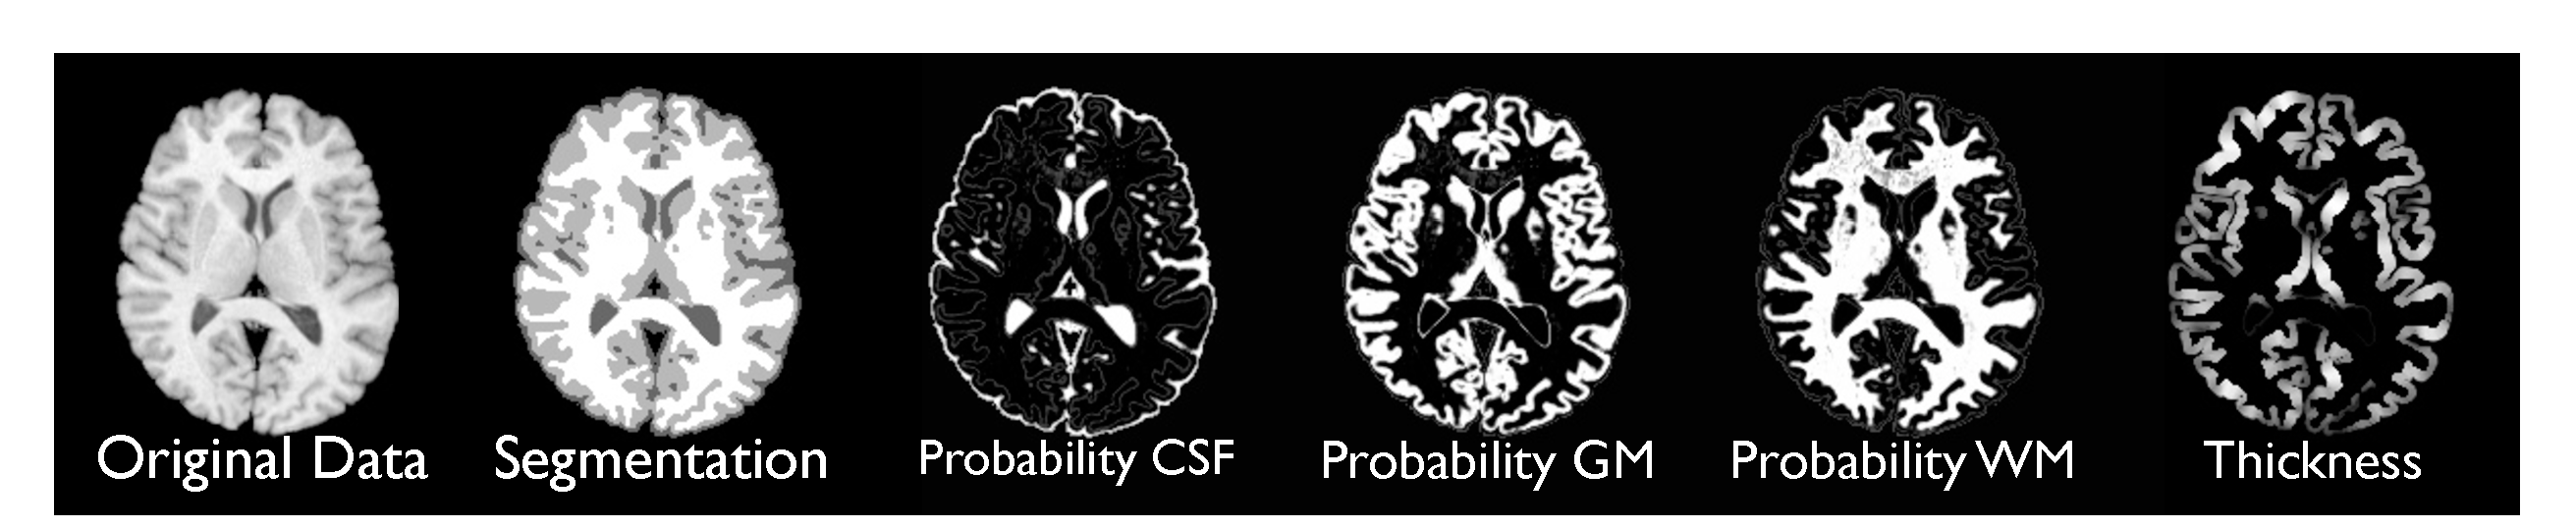
\includegraphics[width=1\textwidth]{Figures/segmentation.pdf} 
\itkcaption[ANTS Segmentation]{ANTS provides basic 
Markov Random Field regularized Gaussian model tissue segmentation. 
The ANTS program N3BiasFieldCorrection is very valuable as preprocessing 
for this naive approach to segmentation.   The last panel -- far right -- 
shows the thickness derived from the white matter and gray matter 
probabilities where a prior on thickness was used to prevent thickness
overestimation.   Thickness was derived with DiReCT \cite{Das2009}, a software 
tool available in binary form only -- a future release may provide code.  
}
\end{figure}
\subsection{Prior and Template-based Image Segmentation}
The same algorithm may be augmented 
to perform Prior-based segmentation.  
\begin{verbatim}
ImageMath 2 r16sliceprior.nii Segment r16slice.nii 4 0.5 
   csfprior.nii wmprior.nii  gmprior.nii 
% output = r16sliceprior_seg.nii  r16sliceprior_prob_0.nii  
% r16sliceprior_prob_1.nii  r16sliceprior_prob_2.nii .  
\end{verbatim}
The parameter \verb 4 indicates 3 tissues plus background are sought.  The \verb 0.5 indicates 
we weight the priors equally as the data term and use a spatially varying set of Gaussians 
to estimate the segmentation.  In this way, data from the priors may be used to modify 
and guide the segmentation in a locally varying way, accomodating for both inhomogeneity 
and the different imaging signature that different tissues provide.   Prior images should be 
of the same size and dimension as the input data and should have intensities in the range $[0,1]$.
\begin{figure}
\label{fig:seg2}
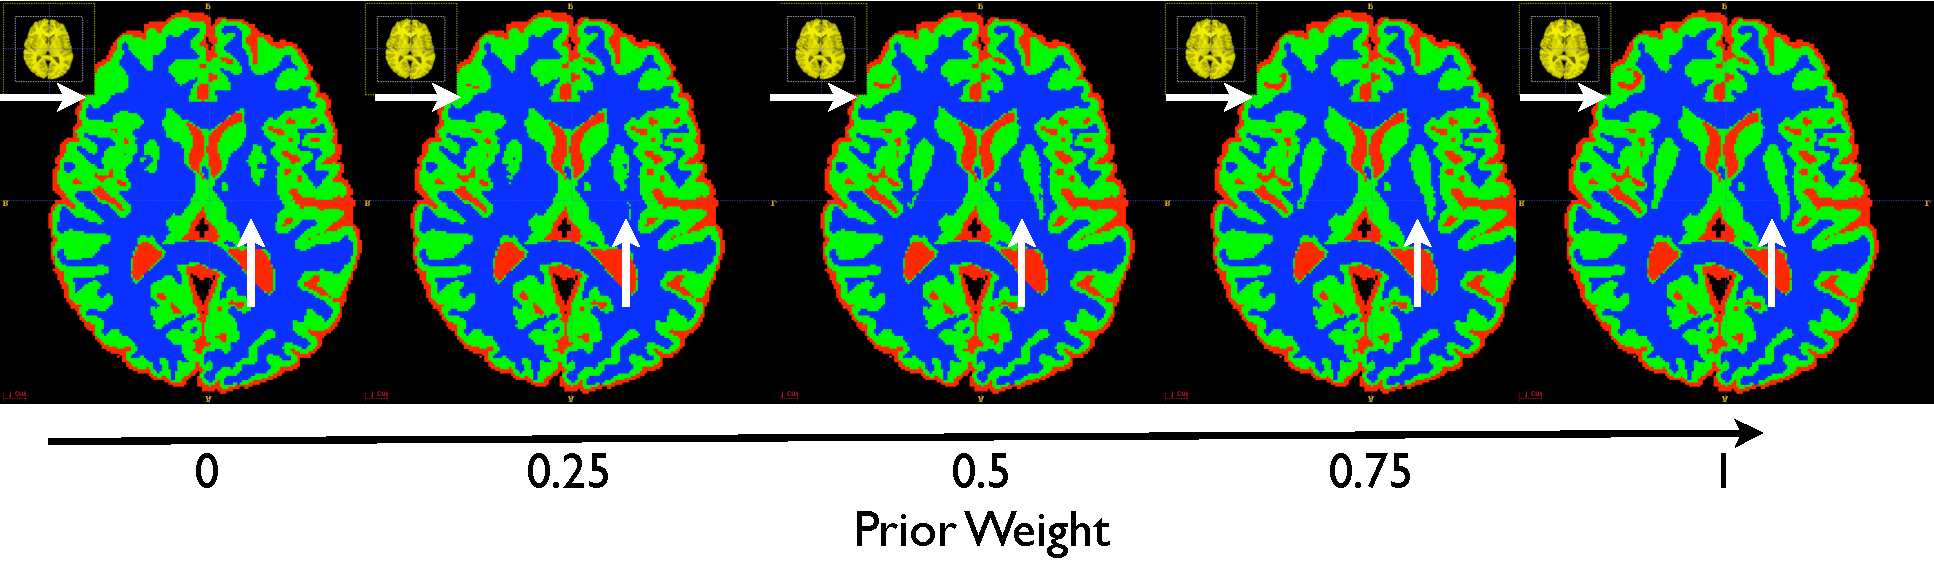
\includegraphics[width=1\textwidth]{Figures/segmentation2.pdf}
\itkcaption[ANTS Segmentation]{ANTS extends basic Markov Random Field
  regularized Gaussian model tissue segmentation to include priors,
  which allow spatially varying tissue models to determine
  segmentation.  The ANTS program N3BiasFieldCorrection is less
  critical as preprocessing when using this approach to segmentation.
  Here, we see the improvement in segmentation as the locally varying 
  prior models are weighted more heavily.  
  The last panel -- far right -- shows the segmentation derived from
  data driven with an initialization founded purely on prior models 
  based on template mapping.  The prior model brings out the caudate 
and some CSF -- highlighted by arrows -- as their weight increases. 
}
\end{figure}
\subsection{Cortical Thickness}
Two forms of cortical thickness estimation from probability maps are available 
in ANTS: first, the traditional Laplacian cortical thickness estimation and, second, 
the more recently developed Diffeomorphic Registration-based Cortical Thickness 
(DiReCT) \cite{Das2009}.  Both methods estimate thickness of an object 
from probability or binary images that define object boundaries.  This tool 
is mainly of interest in brain mapping and cardiac imaging for morphometric 
studies.  Cortical thickness, for instance, is known to correlate with language 
development and IQ in adolescents.  
  
\subsection{User/Label-Guided Normalization for Hippocampus Mapping}
See the link for details on hippocampus labeling:
\href{http://picsl.upenn.edu/ANTS/hipptutorial.php}{http://picsl.upenn.edu/ANTS/hipptutorial.php}.
\noindent{\bf Expectation-Based Point-Set Registration.}
Here, we apply the expectation-based point set registration method 
for mapping labeled points sets.   ITK-SNAP may be used to label 
images and exported segmentation images may be input to the 
PSE metric below, as labeled data.  The Frown and Smile data is used 
as example.  This data is available in the 
ANTS/Examples/Data/ directory.
\begin{figure}
\label{fig:frown}
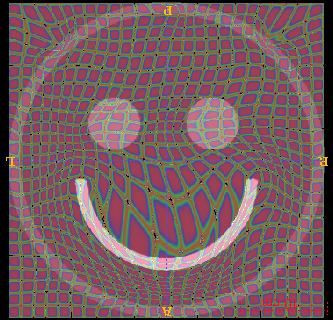
\includegraphics[width=0.45\textwidth]{Figures/frowntosmile.png}
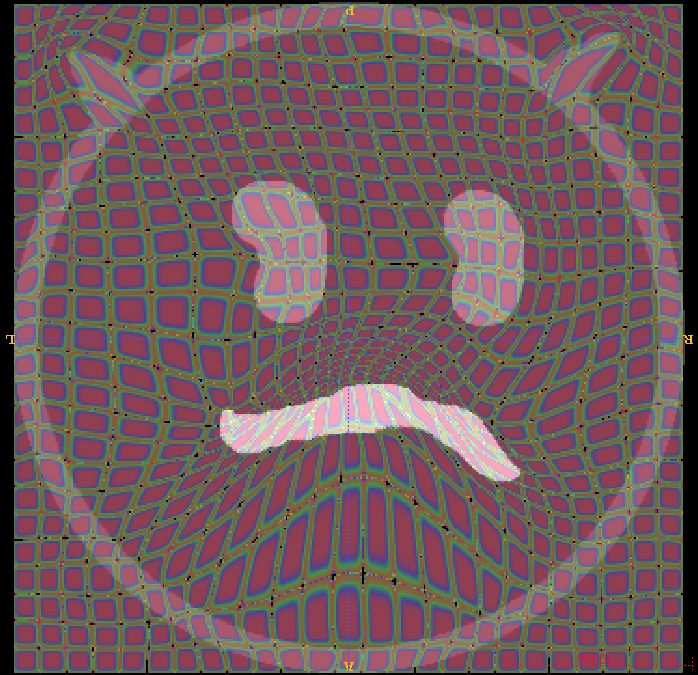
\includegraphics[width=0.45\textwidth]{Figures/smiletofrown.png}
\itkcaption[Frown To Smile]{Expected output for the frown to smile 
shows a smooth, though large deformation.  The grids are overlaid on 
the deformed images. }
\end{figure}
\begin{verbatim}
ANTS 2 -o PSEtest  -i 91x70x55x40x30  -r Gauss[3,0.] -t SyN[0.2]
   -m  PSE[Frown.nii,Smile.nii,Frown.nii,Smile.nii,0.75,0.1,11,0,10] 
   -m  MSQ[Frown.nii,Smile.nii,1,0]    --number-of-affine-iterations 0 

WarpImageMultiTransform  2 Frown.nii FrownToSmile.nii -R Smile.nii
   -i PSEtestAffine.txt PSEtestInverseWarp.nii 

WarpImageMultiTransform  2 Smile.nii SmileToFrown.nii -R Frown.nii 
    PSEtestWarp.nii PSEtestAffine.txt 

CreateWarpedGridImage 2 PSEtestInverseWarp.nii grid1.nii
CreateWarpedGridImage 2 PSEtestWarp.nii grid2.nii
\end{verbatim}
This example should run on the downloaded ANTS data so you may see the results.


%\input{ANTSLabeledDataExample}
%\input{ANTSMaskedImageRegistrationExample}

\section{Application to Studies}
\subsection{Brain Mapping in the Presence of Lesions}
Many cases violate the basic assumption of a one-to-one mapping from a
template image to a target image. Brain lesions caused by stroke or
traumatic brain injury are a common instance of this.

The ANTS toolkit handles this situation by a constrained cost-function
masking approach. In short, the mapping within an excluded region (as
determined by an inclusive mask) is determined by the solution outside
of the region. To achieve this with ANTS, one would use a call similar
to this:
\begin{verbatim}
ANTS 3 -m PR[tp22_s1.nii,template.nii.gz,1,4] -i 50x20x0
   -o tp22map -t SyN[0.5] -x mask.nii.gz -r Gauss[3,0] 
\end{verbatim}
The additional parameter needed for this approach 
is the \verb -x ~ \verb mask.nii.gz ~ which 
is the mask defined in the "fixed" (or individual) image space.  
Mask values above 0.5 are considered non-outlier or non-lesioned regions.
The labeling may be performed with ITK-SNAP. 
Figure~\ref{fig:lesion} illustrates the approach.
\begin{figure}
\label{fig:lesion}
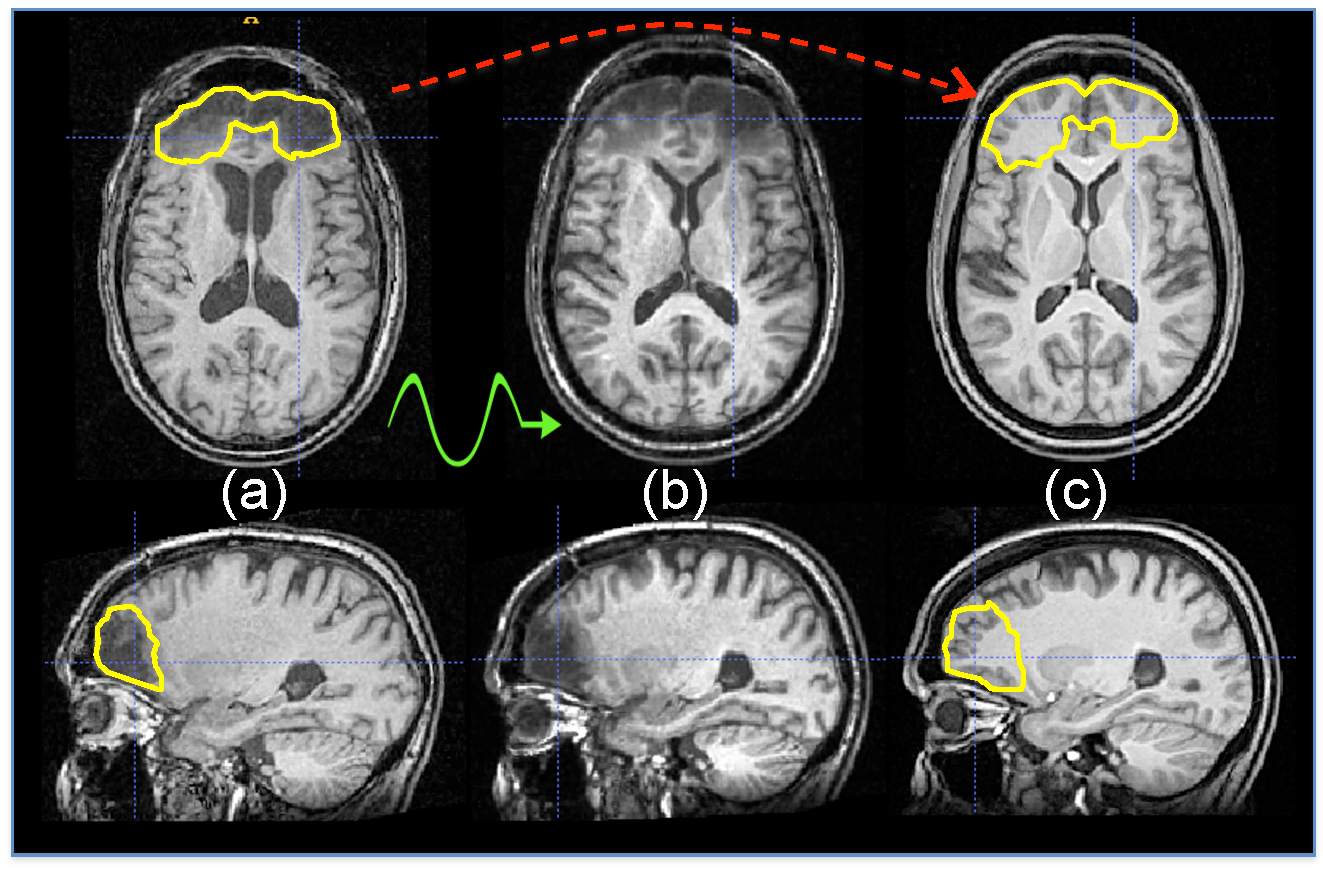
\includegraphics[width=1\textwidth]{Figures/lesionstudy.pdf}
\itkcaption[ANTS Lesions]{Here, we see a semi-automated approach for lesion analysis
based on diffeomorphic normalization.  The user outlines the lesion
site in the subject space, as shown in (a).  Diffeomorphic mapping is
then used to deform the subject image in (a) into the space of the
reference template.  The deformed subject is shown in panel (b).
Panel (c) shows the reference template space with the estimated
position of the subject's lesion overlaid on the healthy tissue of the
template.  This approach enables one to compare the subject image
against prior information stored in the template space such as
anatomical labels or statistics on the appearance of lesioned and/or
normal tissue.}
\end{figure}
Once the ANTS mapping is solved, 
one is able to estimate the location of the lesion in the template space by mapping the inverse lesion mask to the template.
To take the negative image of the inclusive mask 
and warp the mask to the template :
\begin{verbatim}
ImageMath 3 lesionmask.nii.gz Neg inclusivemask.nii.gz
WarpImageMultiTransform 3 lesionmask.nii.gz lesiontotemplate.nii.gz 
   -R template.nii.gz -i tp22mapAffine.txt tp22mapInverseWarp.nii
\end{verbatim}
More details on this approach are being prepared for publication.
See also: \verb http://www.ncrrn.org/papers/methodology_papers/sp_norm_kim.pdf .

\subsection{Statistical Mapping with ANTS: Morphometry, Function, Jacobian, Thickness}
ANTS has been applied in a wide array of imaging studies
\cite{Avants2009a,Avants2009b,Avants2009,Das2009,Klein2009,Massimo2009,Pluta2008,Tustison2009,Yushkevich2009,Avants2008c,Avants2008b,M.Grossman10282008,Kim2008,Simon2008,Sun2008,Yushkevich2008,Aguirre2007,Avants2007,Avants2007i}.
All of these studies benefit in some way from normalization whether the topic is cortical
thickness, Jacobian-based morphometry, volumetric morphometry or functional studies. 
From a broad perspective, each of these applications requires the same steps:
\begin{enumerate}
\item Preprocess images -- bias correction, segmentation, etc.  Potentially construct an optimal template. 
\item Normalize images -- run \verb ants.sh ~ to map a population of images to a template and store the deformations. 
\item Derive any data from the deformation that may be necessary, e.g. the log-Jacobian.
\item Apply the warp to any images one may want to analyze in template space.  
\item Perform statistics in template space over the region of interest, e.g. all cortex. 
\end{enumerate}
We now illustrate this procedure using ANTS tools and example images from ANTS/Examples/Data. 
The expected output is in figure~\ref{fig:morph}.
\begin{verbatim}
1.  ImageMath 2 r64slice.nii Segment r64slice.nii 4 0
1.  ImageMath 2 r16slice.nii Segment r16slice.nii 4 0
2.  sh ants.sh 2 r16slice.nii r64slice.nii SPM 100x100x100
3.  SmoothImage 2 r64slice_prob_1.nii  1. r64slice_prob_1.nii  
3.  WarpImageMultiTransform 2 r64slice_prob_1.nii  r64slice_prob_1_norm.nii
     -R r16slice.nii SPMWarp.nii SPMAffine.txt 
3.  ANTSJacobian 2 SPMWarp.nii SPM 1  # take the log
4.  ImageMath 2 SPMlogjacobianmask.nii m SPMlogjacobian.nii r64slice_prob_1_norm.nii
5.  Repeat for a population and run statistics on log jacobians.
\end{verbatim}
\begin{figure}
\label{fig:morph}
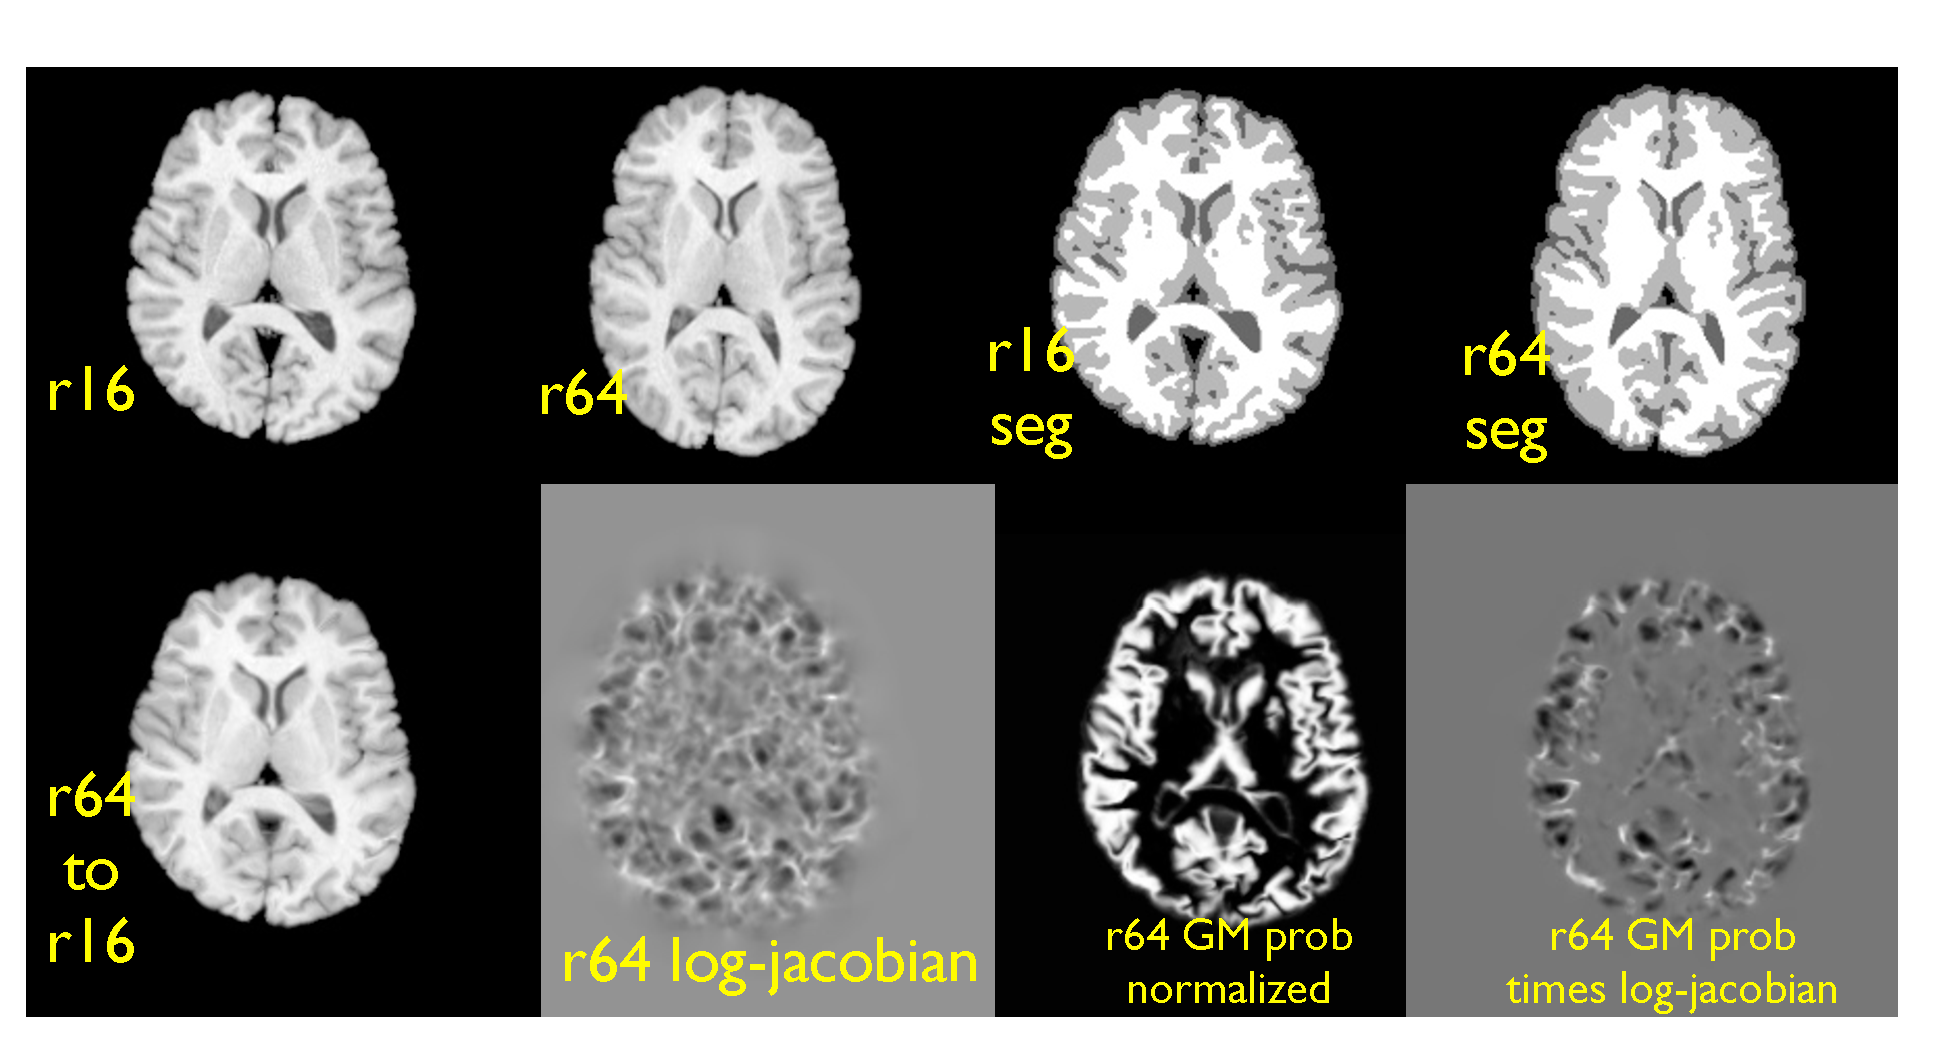
\includegraphics[width=1\textwidth]{Figures/morphometry.pdf}
\itkcaption[ANTS Morphometry]{The output from the ANTS morphometry example.}
\end{figure}
This example uses a standard Jacobian-based approach to morphometry.
Here, we use the log-Jacobian because it is symmetric about zero and
mask with the gray matter segmentation to restrict the analysis to the
cortex.  The Jacobian is discussed in figure~\ref{fig:inv} and visualization of
the Jacobian is shown in figure~\ref{fig:jac}.  This Jacobian comes
from the mapping shown in figure~\ref{fig:large}.
\begin{figure}
\label{fig:jac}
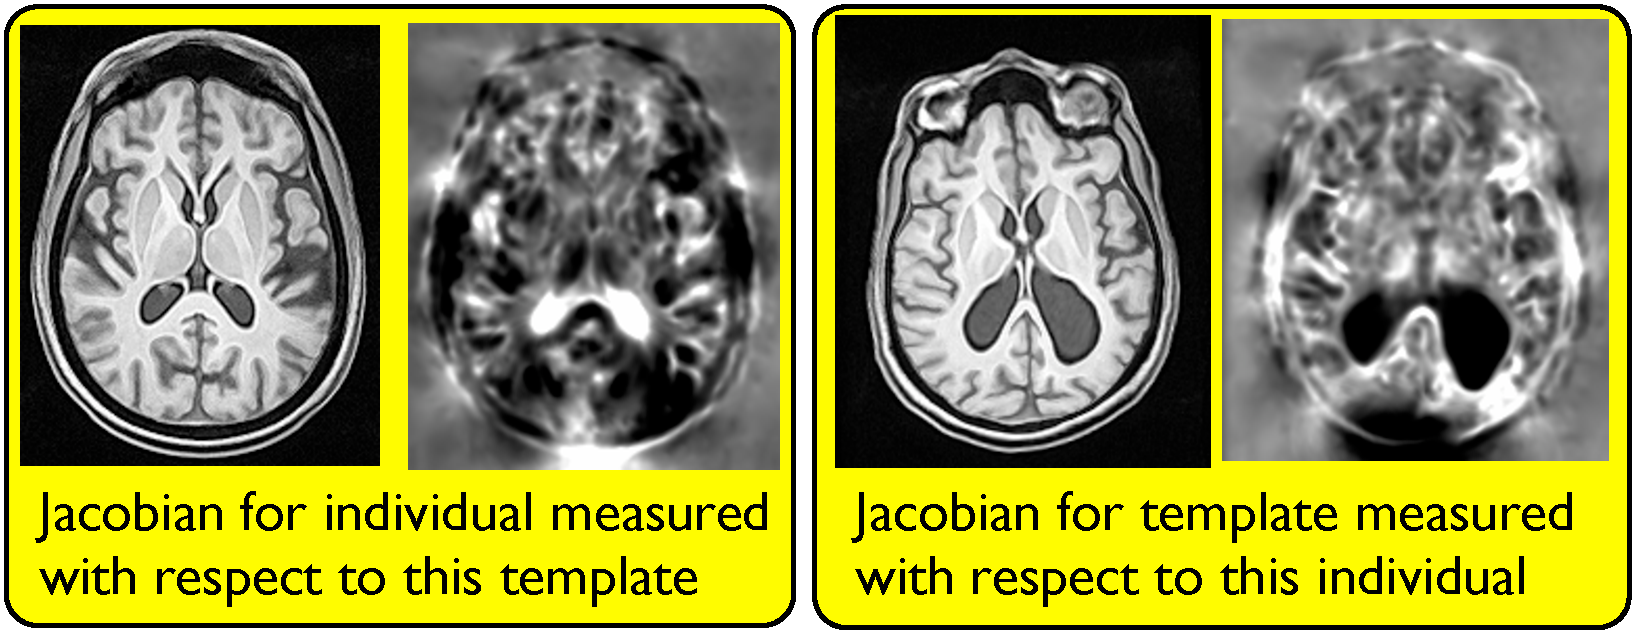
\includegraphics[width=1\textwidth]{Figures/Jacobian.pdf}
\itkcaption[ANTS Jacobian]{The Jacobian: Note that the bright values
  in the template image ventricles (left) indicate that the ventricles
  are relatively larger in the subject image. Similarly, the dark
  jacobian values in the individual image show that the template has
  smaller ventricles. This example is described on the large
  deformation page Large Def. Once one gains the Jacobian (or more
  appropriately, the log-Jacobian), then one may compute statistics
  across the population.}
\end{figure}
Similar analyses may be performed on thickness images, functional 
images or fractional anisotropy images derived from the diffusion 
tensor modality.  In all these cases, steps similar to those above 
would be performed.  

\subsection{Statistics with ANTS and ``R''}
{\bf R} is an open-source, cutting-edge statistical package 
used by statisticians world-wide.   ANTS is designed to 
interface with {\bf R} via an ImageMath tool that converts 
image sets into an {\bf R} compatible format.  
Three steps are required.  First, convert image data into 
vector and matrix formats through a mask of your statistical 
region of interest.  Second, read that data into {\bf R} and 
run your statistics.  Third, write out the data from {\bf R} and 
convert back to an image.  Here are the steps, in code examples,
\begin{enumerate}
\item Create a vector for your output: 
\begin{verbatim} 
ImageMath 3 testresultvec.nii ConvertImageSetToMatrix 1 mask.nii image1.nii
\end{verbatim}
Here, we assume all images are called image1.nii, image2.nii, ... , imageN.nii so we 
can use a wildcard to pass to ImageMath and 
create a matrix for all your input data: 
\begin{verbatim} 
 ImageMath 3 datamatrix.nii ConvertImageSetToMatrix 1 mask.nii image*.nii 
\end{verbatim}
\item   Run {\bf R} by reading your data above, performing whatever statistics you want and then 
writing out.  
\item   Convert the test result back to an image.  
\begin{verbatim} 
ImageMath 3 testresult.nii ConvertVectorToImage mask.nii testresultvec.nii
\end{verbatim}
\end{enumerate}
Most statistical requirements may be met with this setup. 
\section{Dependencies and Related Software}
\subsection{Dependencies and Compilation}
ANTS depends on the most recent version of the Insight ToolKit (ITK)
-- www.itk.org.   File types that may be read and written are 
all of those available in itk and a few more \href{http://picsl.upenn.edu/ANTS/ioants.php}{http://picsl.upenn.edu/ANTS/ioants.php}.

ANTS and ITK are both compiled through pointing CMake -- www.cmake.org
-- to a CMakeLists.txt file.  The ANTS CMakeLists.txt is in the
Examples directory.  

See below for more details on compilation and binaries: \newline
\href{http://picsl.upenn.edu/ANTS/download.php}{Compile and download: http://picsl.upenn.edu/ANTS/download.php}.
We maintain a dashboard to give users an idea of what to expect 
from compilation:\newline
\href{http://picsl.upenn.edu/cdash/index.php?project=ANTS}{http://picsl.upenn.edu/cdash/index.php?project=ANTS}


\subsection{Visualization and Quantification of ANTS Results}
Use \href{www.itksnap.org}{itk SNAP : www.itksnap.org } or mricro / mricron for viewing
images.  The ANTS program StackSlices can be used to conveniently scan
through a dataset in any of its axes.  It is useful for checking both
input data quality and output normalization quality.  MeasureImageSimilarity 
will supply numerical measures of image similarity via three different metrics. 

\subsection{Statistics Beyond ANTS}
Use SPM, {\bf R} or npm (from Chris Rorden's mricron) for computing population statistics.

\subsection{Pipelining with ANTS}
Use PipeDream for automating large-scale processing:\newline
\href{https://sourceforge.net/projects/neuropipedream/}{PipeDream
  Homepage :
  https://sourceforge.net/projects/neuropipedream/} \newline PipeDream
is integrated with ANTS and automates more complex studies such as
multivariate diffusion tensor and T1 cortical thickness studies,
longitudinal mapping and reconstruction of nifti images from Dicom.



%%%%%%%%%%%%%%%%%%%%%%%%%%%%%%%%%%%%%%%%%
%
%  Insert the bibliography using BibTeX
%
%%%%%%%%%%%%%%%%%%%%%%%%%%%%%%%%%%%%%%%%%

\bibliographystyle{plain}
\bibliography{ants}


\end{document}

